\documentclass[11pt]{article}

\usepackage[a4paper,margin=27mm]{geometry}
\usepackage[T1]{fontenc}
\usepackage{lmodern}
\usepackage{microtype}
\usepackage{amsmath,amssymb,mathtools}
\usepackage{array,booktabs,longtable,tabularx}
\usepackage{enumitem}
\usepackage{graphicx}
\usepackage{tikz}
\usetikzlibrary{arrows.meta,calc,fit,positioning,shapes.geometric}
\usepackage{xurl}
\usepackage[hidelinks]{hyperref}

\setlength{\emergencystretch}{3em}
\graphicspath{{figures/}{../figures/}}
\newcolumntype{Y}{>{\raggedright\arraybackslash}X}
\newcolumntype{L}[1]{>{\raggedright\arraybackslash}p{#1}}
\tikzset{
  protocolbox/.style={
    draw,
    rounded corners,
    align=center,
    minimum height=8mm,
    text width=31mm,
    inner sep=2mm
  },
  wideprotocolbox/.style={
    protocolbox,
    text width=43mm
  },
  protocolarrow/.style={-{Latex[length=2.2mm]},thick},
  evidencebox/.style={protocolbox,fill=blue!8,draw=blue!55!black},
  plannedbox/.style={protocolbox,fill=orange!10,draw=orange!70!black},
  stopbox/.style={protocolbox,fill=red!8,draw=red!65!black},
  verifybox/.style={protocolbox,fill=green!8,draw=green!55!black}
}

\title{Research Protocol:\\Periodic-2D Rank-Defect Extraction and Finite-Domain Sensitivity}
\author{Project Koios}
\date{Calculation-owned protocol, version 7}

\begin{document}
\maketitle

\begin{abstract}
This protocol defines a controlled synthetic research program for extracting,
representing, reducing, and comparing defects in finite representations of periodic
two-dimensional operators.  It replaces opaque lettered phases with five named
workstreams: Folding and Null-Alignment Controls, Onsite Extraction and Covariance
Controls, Defect-Model Discrimination, Finite-Domain Sensitivity, and
Composite-Subspace Extension.  The active evidence consists of one authored,
dimensionless rank-one folding/null result, one exact accepted-historical-synthetic
parent qualification, and one execution-free finite-domain case inventory.  No
physical/material parent, convergence, uncertainty, Quantum ESPRESSO, Wannier90, or
external-computation claim follows from this document.
\end{abstract}

\noindent\textbf{Keywords:} periodic defects; finite periodic operators; boundary
twists; gauge alignment; model discrimination; finite-domain sensitivity

\tableofcontents
\clearpage
\listoffigures
\clearpage

\section{Protocol status}

\begin{center}
\small
\begin{tabularx}{\textwidth}{>{\raggedright\arraybackslash}p{0.34\textwidth}Y}
\toprule
\textbf{Field} & \textbf{Value} \\
\midrule
Protocol version & 7 \\
Calculation owner & \path{calculations/periodic2d_rank_defect/} \\
Scientific dimension & Two periodic lattice dimensions \\
Active retained rank & One scalar state per primitive cell \\
Current evidence & Authored Folding and Null-Alignment Controls result, accepted-historical-synthetic parent qualification, and version-2 execution-free Finite-Domain Sensitivity inventory \\
Protected or external execution authorized by this protocol & No \\
Accepted-parent operator production authorized by this protocol & No \\
Material, silicon, dopant, convergence, or uncertainty claim & None \\
\bottomrule
\end{tabularx}
\end{center}

The removed \path{calculations/research-monograph/impurity-defect-2d/} tree is a
provenance and design donor available through Git history.  It is not restored as an
active runner, calculation owner, authorization mechanism, or source import path.
The current retained folding/null result is an authored, dimensionless synthetic
numerical result.  The current finite-domain package is a version-2 case inventory with execution status
\texttt{not\_executed}; its version-1 predecessor remains immutable retained evidence.  This protocol does not retroactively strengthen, seal, or
scientifically validate either package.

\section{Research objective}

The program asks when a defect operator can be meaningfully extracted, represented,
reduced, and compared after the parent and candidate operators have been placed in the
same finite state space.  The research questions are:

\begin{enumerate}[leftmargin=*]
  \item Does finite Bloch folding reproduce the declared primitive scalar operator
    under the selected boundary-twist convention?
  \item Can a known translation, site-phase gauge, and scalar energy-reference change
    be removed before subtraction without leaving a false defect?
  \item Which incompatibilities must stop extraction rather than produce an operator
    residual?
  \item Can scalar onsite, directional nearest-neighbour, and finite-range nonlocal
    defects be distinguished by a frozen nested model hierarchy?
  \item Are symmetry and orientation conclusions covariant under the correct
    transformation of geometry, defect support, parent identity, and boundary twist?
  \item How do finite area, fixed-area shape, orientation, and boundary phase affect
    operator, spectral, and state diagnostics when those channels remain separate?
  \item What is the smallest support-unaliased square cell whose extracted defect
    behaves as an isolated localized perturbation rather than a strongly coupled
    periodic array of defect images?
  \item In a separately reviewed branch, can the same contracts be extended to a
    composite retained subspace without treating arbitrary vectors inside degenerate
    clusters as observables?
\end{enumerate}

Algebraic identities may be verification criteria.  Expected physical trends are not
verification oracles.  Failed, nonmonotone, unresolved, and no-bound-state outcomes
remain evidence.

\section{Scientific and software boundaries}

This protocol distinguishes:

\begin{enumerate}[leftmargin=*]
  \item the periodic parent model expressed through hopping coefficients;
  \item the mathematical parent or defect operator on a declared finite periodic state
    space;
  \item a finite matrix representation in a declared ordering and boundary gauge; and
  \item analysis records derived from compatible represented operators.
\end{enumerate}

A matrix is not subtracted from another matrix merely because their dimensions agree.
Geometry, represented rank, basis identity, site correspondence, boundary twist, gauge,
energy reference, and units must first be identified and reconciled.

Reusable lattice, twist, represented-operator, seam, gauge-bridge, and defect mechanics
belong to PhysKit or maintained \path{ksdft2effmass.solidstate} and periodic owners.
This calculation family owns adopted case inventories, campaign policy, thresholds,
provenance bindings, retained results, and calculation-local composition.

The protocol excludes Quantum ESPRESSO or Wannier90 execution; remote, cluster, cloud,
or network computation; accepted-parent execution before the periodic-2D parity gate;
DFT or material claims; spin or SOC conclusions; construction-mesh convergence;
uncertainty quantification; post hoc threshold selection; and interpreting a software
pass as scientific validation.

\section{Represented spaces and conventions}

For a finite shape $N_x\times N_y$, the active scalar state space is
\begin{equation}
  \mathcal H_{N_x,N_y}=\mathbb C^{N_xN_y}.
\end{equation}
Sites are integer pairs $(x,y)$ with $x$ outer and $y$ inner, so the scalar flat index is
$xN_y+y$.  The retained rank is one per primitive cell.  A future composite branch must
state its exact rank and orbital ordering in a separate revision.

Boundary twists are measured in turns,
$\boldsymbol\phi=(\phi_x,\phi_y)$.  A hopping displacement crossing $q_x$ and $q_y$
periodic boundaries receives the quotient-seam phase
\begin{equation}
  \exp\!\left[2\pi i(q_x\phi_x+q_y\phi_y)\right].
\end{equation}
The finite folding matrix is
\begin{equation}
  F_{(x,y),(j_x,j_y)}=
  (N_xN_y)^{-1/2}
  \exp\!\left[
    2\pi i\left(
      \frac{j_x+\phi_x}{N_x}x+
      \frac{j_y+\phi_y}{N_y}y
    \right)
  \right].
\end{equation}

The active Folding and Null-Alignment Controls workstream is dimensionless and uses the
energy reference \path{authored-folding-null-zero}.  Historical successor selections
use $E_G=1$, $G=1$, and $a=2\pi$ only as synthetic reporting units.  They are not
material parameters.

\section{Complete mathematical formulation}

This section records the mathematics used by the active folding/null calculation and
the mathematics frozen for the unexecuted successor workstreams.  A prospective
definition below is not evidence that its operator, spectrum, or diagnostic has been
calculated.

\subsection{Infinite periodic scalar parent}

Let $\mathcal S\subset\mathbb Z^2$ be a finite hopping support and let
$h_{\mathbf R}\in\mathbb C$ satisfy
\begin{equation}
  h_{-\mathbf R}=h_{\mathbf R}^{*}.
\end{equation}
The translation-invariant scalar operator is represented by
\begin{equation}
  H_{\mathbf n,\mathbf n+\mathbf R}=h_{\mathbf R},
  \qquad \mathbf n\in\mathbb Z^2,
  \quad \mathbf R\in\mathcal S.
\end{equation}
With reciprocal coordinates measured in turns, the primitive Bloch energy is
\begin{equation}
  \varepsilon(\mathbf k)
  =\sum_{\mathbf R\in\mathcal S}
    h_{\mathbf R}\exp\!\left(2\pi i\,\mathbf k\cdot\mathbf R\right).
  \label{eq:primitive-bloch-energy}
\end{equation}
Hermiticity makes \eqref{eq:primitive-bloch-energy} real.  For the active authored
nearest-neighbour parent,
\begin{equation}
  \varepsilon(k_x,k_y)
  =0.20-0.20\cos(2\pi k_x)-0.16\cos(2\pi k_y).
  \label{eq:authored-parent-dispersion}
\end{equation}
Equation~\eqref{eq:authored-parent-dispersion} is active synthetic control mathematics,
not a material dispersion.

\subsection{Finite periodic quotient and seam construction}

Write
\begin{equation}
  \Lambda_{\mathbf N}
  =\mathbb Z_{N_x}\times\mathbb Z_{N_y},
  \qquad \mathbf N=(N_x,N_y).
\end{equation}
For a source $\mathbf n\in\Lambda_{\mathbf N}$ and displacement $\mathbf R$, Euclidean
integer division uniquely gives
\begin{equation}
  \mathbf n+\mathbf R
  =\overline{\mathbf n+\mathbf R}
   +\mathbf q(\mathbf n,\mathbf R)\odot\mathbf N,
  \label{eq:quotient-decomposition}
\end{equation}
where the barred coordinate lies in the finite fundamental domain and $\odot$ denotes
componentwise multiplication.  The quotient-seam matrix is
\begin{equation}
  H^{\mathrm{seam}}_{\mathbf n,
    \overline{\mathbf n+\mathbf R}}(\boldsymbol\phi)
  \mathrel{+}=
  h_{\mathbf R}\exp\!\left[
    2\pi i\,\mathbf q(\mathbf n,\mathbf R)\cdot\boldsymbol\phi
  \right].
  \label{eq:seam-matrix}
\end{equation}
Distinct primitive displacements that have the same finite source and target are summed
in the same matrix entry.  Such summation is exact quotient arithmetic; it is also the
mechanism by which small cells alias distinct support terms.

For a localized bond whose declared start may itself lie outside the fundamental
domain, let $\mathbf q_s$ and $\mathbf q_t$ be the source and target quotient integers.
Its phase is
\begin{equation}
  \exp\!\left[
    2\pi i(\mathbf q_t-\mathbf q_s)\cdot\boldsymbol\phi
  \right].
  \label{eq:localized-seam-phase}
\end{equation}

\begin{figure}[htbp]
  \centering
  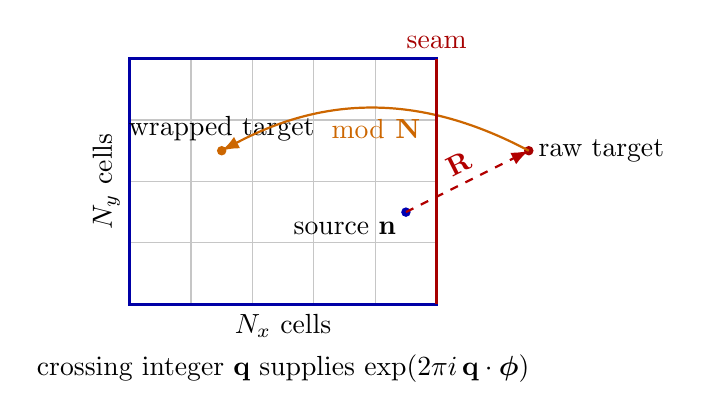
\begin{tikzpicture}[scale=0.78]
    \draw[step=1,gray!45,thin] (0,0) grid (5,4);
    \draw[blue!65!black,very thick] (0,0) rectangle (5,4);
    \node[below] at (2.5,0) {$N_x$ cells};
    \node[rotate=90,above] at (0,2) {$N_y$ cells};
    \fill[blue!70!black] (4.5,1.5) circle (2.2pt);
    \node[below left] at (4.5,1.5) {source $\mathbf n$};
    \fill[orange!80!black] (1.5,2.5) circle (2.2pt);
    \node[above] at (1.5,2.5) {wrapped target};
    \coordinate (raw) at (6.5,2.5);
    \fill[red!65!black] (raw) circle (2.2pt);
    \node[right] at (raw) {raw target};
    \draw[protocolarrow,red!70!black,dashed]
      (4.5,1.5) -- node[above,sloped] {$\mathbf R$} (raw);
    \draw[protocolarrow,orange!80!black,bend right=28]
      (raw) to node[below] {$\bmod\ \mathbf N$} (1.5,2.5);
    \draw[red!65!black,very thick] (5,0) -- (5,4);
    \node[red!65!black,above] at (5,4) {seam};
    \node[align=center] at (2.5,-1.05)
      {crossing integer $\mathbf q$ supplies
       $\exp(2\pi i\,\mathbf q\cdot\boldsymbol\phi)$};
  \end{tikzpicture}
  \caption{Quotient-seam construction.  The raw target is reduced to the fundamental
  domain, while the discarded quotient integer is retained in the boundary phase.}
  \label{fig:quotient-seam-schematic}
\end{figure}

\subsection{Finite Bloch folding}

The allowed folded momenta are
\begin{equation}
  \mathbf k_{\mathbf j}(\boldsymbol\phi)
  =\left(
    \frac{j_x+\phi_x}{N_x},
    \frac{j_y+\phi_y}{N_y}
  \right),
  \qquad
  j_a\in\{0,\ldots,N_a-1\}.
\end{equation}
The folding matrix is unitary when
\begin{equation}
  F^{\dagger}F=FF^{\dagger}=I,
\end{equation}
and exact folding requires
\begin{equation}
  F^{\dagger}H^{\mathrm{seam}}(\boldsymbol\phi)F
  =\operatorname{diag}_{\mathbf j}
    \varepsilon\!\left(\mathbf k_{\mathbf j}(\boldsymbol\phi)\right).
  \label{eq:finite-folding-identity}
\end{equation}
The active calculation retains maximum-entry defects for unitarity, Hermiticity,
off-diagonal folding, primitive-energy reconstruction, and sorted-spectrum agreement.
For a matrix $A$ these norms are
\begin{align}
  \lVert A\rVert_{\max} &= \max_{ij}|A_{ij}|, \\
  \lVert A\rVert_F &= \sqrt{\operatorname{Tr}(A^{\dagger}A)}.
\end{align}

\subsection{Uniform-link gauge and explicit bridge}

For an unreduced twist lift $\widetilde{\boldsymbol\phi}$, a centered uniform-link route
distributes the phase across every bond.  In the adopted convention a hopping
$\mathbf R$ receives
\begin{equation}
  \exp\!\left[
    2\pi i\left(
      \frac{R_x\widetilde\phi_x}{N_x}
      +\frac{R_y\widetilde\phi_y}{N_y}
    \right)
  \right].
  \label{eq:uniform-link-phase}
\end{equation}
The site-diagonal bridge is
\begin{equation}
  D_{\mathbf n\mathbf n}(\widetilde{\boldsymbol\phi})
  =\exp\!\left[
    2\pi i\left(
      \frac{n_x\widetilde\phi_x}{N_x}
      +\frac{n_y\widetilde\phi_y}{N_y}
    \right)
  \right],
\end{equation}
with route equivalence
\begin{equation}
  H_{\mathrm{seam}}(\widetilde{\boldsymbol\phi}\bmod1)
  =D(\widetilde{\boldsymbol\phi})
   H_{\mathrm{uniform}}(\widetilde{\boldsymbol\phi})
   D(\widetilde{\boldsymbol\phi})^{\dagger}.
  \label{eq:gauge-bridge}
\end{equation}
The two constructions are separate implementations.  Equation~\eqref{eq:gauge-bridge}
is a gauge-equivalence test, not an averaging rule.

\subsection{Localized perturbation operators}

A scalar onsite perturbation at site $\mathbf r_0$ is
\begin{equation}
  \Delta_{\mathrm{on}}(v,\mathbf r_0)
  =v\,|\mathbf r_0\rangle\langle\mathbf r_0|.
\end{equation}
A Hermitian bond perturbation with displacement $\mathbf d$ is
\begin{equation}
  \Delta_{\mathrm{bond}}
  =\delta t\,|\mathbf r_0\rangle
    \langle\mathbf r_0+\mathbf d|
   +\delta t^{*}\,|\mathbf r_0+\mathbf d\rangle
    \langle\mathbf r_0|.
  \label{eq:bond-perturbation}
\end{equation}
The frozen directional nearest-neighbour control is the sum of
\eqref{eq:bond-perturbation} for $\mathbf d=(1,0)$ and $(0,1)$ with amplitudes
$+0.04$ and $-0.03$.  The frozen diagonal nonlocal control uses
$\mathbf d=(1,1)$ with amplitude $+0.025$.  These values are synthetic selections.

\begin{figure}[htbp]
  \centering
  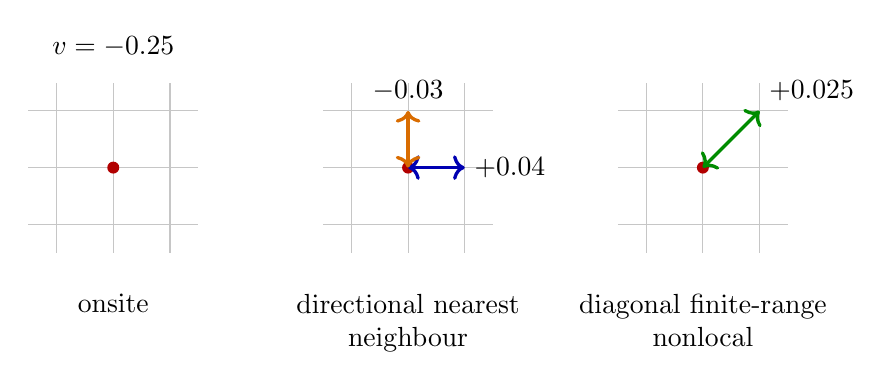
\begin{tikzpicture}[scale=0.72]
    \begin{scope}[xshift=0cm]
      \draw[step=1,gray!45] (-1.5,-1.5) grid (1.5,1.5);
      \fill[red!70!black] (0,0) circle (3pt);
      \node[below=4mm] at (0,-1.5) {onsite};
      \node[above=2mm] at (0,1.5) {$v=-0.25$};
    \end{scope}
    \begin{scope}[xshift=5.2cm]
      \draw[step=1,gray!45] (-1.5,-1.5) grid (1.5,1.5);
      \fill[red!70!black] (0,0) circle (3pt);
      \draw[blue!70!black,very thick,<->] (0,0) -- (1,0);
      \draw[orange!85!black,very thick,<->] (0,0) -- (0,1);
      \node[right] at (1,0) {$+0.04$};
      \node[above] at (0,1) {$-0.03$};
      \node[below=4mm,align=center] at (0,-1.5)
        {directional nearest\\neighbour};
    \end{scope}
    \begin{scope}[xshift=10.4cm]
      \draw[step=1,gray!45] (-1.5,-1.5) grid (1.5,1.5);
      \fill[red!70!black] (0,0) circle (3pt);
      \draw[green!55!black,very thick,<->] (0,0) -- (1,1);
      \node[above right] at (1,1) {$+0.025$};
      \node[below=4mm,align=center] at (0,-1.5)
        {diagonal finite-range\\nonlocal};
    \end{scope}
  \end{tikzpicture}
  \caption{Frozen scalar defect supports.  Every bond term includes its Hermitian
  reverse; colors distinguish terms but do not encode physical orbitals.}
  \label{fig:defect-support-schematic}
\end{figure}

For a model class spanned by represented matrices $B_1,\ldots,B_p$, the least-squares
projection uses the real Frobenius inner product
\begin{equation}
  \langle A,B\rangle_F
  =\operatorname{Re}\operatorname{Tr}(A^{\dagger}B).
\end{equation}
The coefficient vector solves
\begin{align}
  \sum_{b=1}^{p}G_{ab}\alpha_b &= g_a, \\
  G_{ab}&=\langle B_a,B_b\rangle_F,
  \qquad
  g_a=\langle B_a,\Delta\rangle_F,
\end{align}
and the residual is
\begin{equation}
  R_p=\Delta-\sum_{a=1}^{p}\alpha_aB_a.
  \label{eq:model-residual}
\end{equation}
The first frozen class satisfying every applicable residual and support criterion is
selected.  A spectral match alone cannot select a class.

\subsection{Compatibility, alignment, and extraction}

Let $C(H_1,H_2)$ denote the conjunction of equal geometry, represented rank, basis
identity, site correspondence, boundary fiber, energy unit, and a known or declared
energy-reference relation.  Subtraction is defined only when
\begin{equation}
  C(H_{\mathrm{pris}},\widetilde H_{\mathrm{def}})=\mathrm{true}.
\end{equation}
A declared alignment may combine a lattice translation $P_{\mathbf t}$, point-group
permutation $P_M$, site phases $S_{\boldsymbol\theta}$, and, in a composite branch, an
orbital unitary $U$.  Its finite representation is
\begin{equation}
  G=P_M P_{\mathbf t}S_{\boldsymbol\theta}U,
  \qquad G^{\dagger}G=I.
\end{equation}
For scalar rank one, $U=I$.  With scalar energy shift $c$, the extracted perturbation is
\begin{equation}
  \Delta_{\mathrm{rec}}
  =G^{\dagger}(\widetilde H_{\mathrm{def}}-cI)G-H_{\mathrm{pris}}.
  \label{eq:aligned-extraction}
\end{equation}
The active null attack has
\begin{equation}
  G_{\mathbf n+\mathbf t,\mathbf n}
  =\exp\!\left[i(\theta_x n_x+\theta_y n_y)\right],
  \qquad
  \mathbf t=(1,1),
  \quad
  (\theta_x,\theta_y)=(0.137,-0.191),
\end{equation}
and constructs
\begin{equation}
  \widetilde H=GHG^{\dagger}+cI,
  \qquad c=0.137.
\end{equation}
Its exact oracle is $\Delta_{\mathrm{rec}}=0$ up to declared numerical tolerances.

\begin{figure}[htbp]
  \centering
  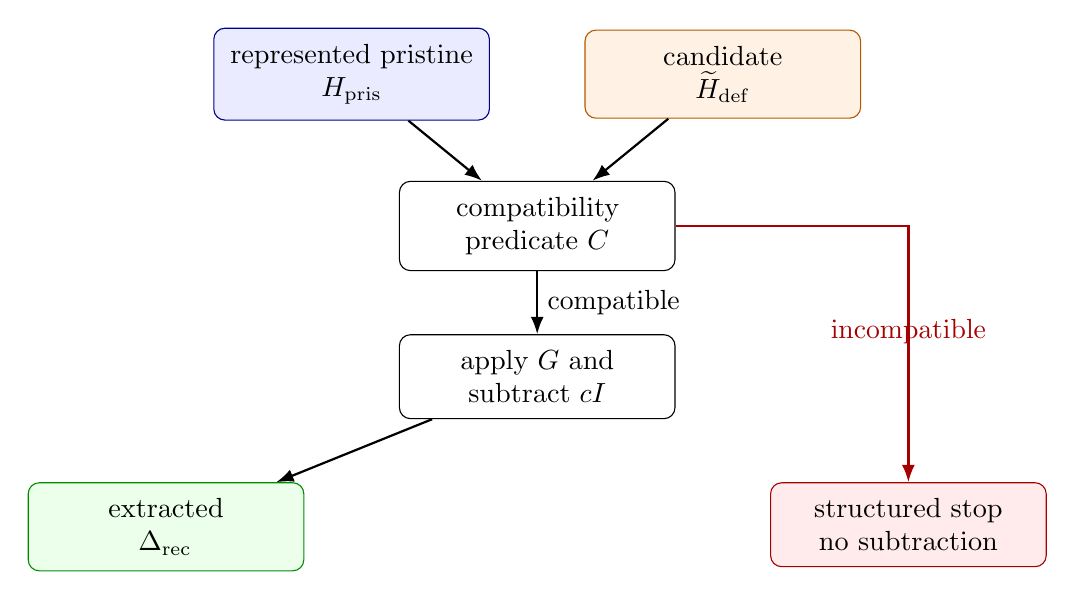
\begin{tikzpicture}[node distance=8mm and 12mm]
    \node[evidencebox] (pristine) {represented pristine\\$H_{\mathrm{pris}}$};
    \node[plannedbox,right=of pristine] (candidate)
      {candidate\\$\widetilde H_{\mathrm{def}}$};
    \node[protocolbox] (compat) at
      ($(pristine.south)!0.5!(candidate.south)+(0,-1.35)$)
      {compatibility\\predicate $C$};
    \node[protocolbox,below=of compat] (align)
      {apply $G$ and\\subtract $cI$};
    \node[verifybox,below left=of align] (delta)
      {extracted\\$\Delta_{\mathrm{rec}}$};
    \node[stopbox,below right=of align] (stop)
      {structured stop\\no subtraction};
    \draw[protocolarrow] (pristine) -- (compat);
    \draw[protocolarrow] (candidate) -- (compat);
    \draw[protocolarrow] (compat) -- node[right] {compatible} (align);
    \draw[protocolarrow] (align) -- (delta);
    \draw[protocolarrow,red!65!black] (compat) -| node[above,pos=0.75]
      {incompatible} (stop);
  \end{tikzpicture}
  \caption{Compatibility-gated extraction.  Matrix dimensions alone never authorize
  subtraction; incompatibility produces a structured stop rather than a residual.}
  \label{fig:alignment-extraction-schematic}
\end{figure}

\subsection{Symmetry and orientation covariance}

For an integer point operation $M$, let $U_M$ be its exact finite-site permutation.
Twists transform as
\begin{equation}
  \boldsymbol\phi' = M\boldsymbol\phi\pmod1.
\end{equation}
An algebraic covariance check has the form
\begin{equation}
  H_{p'}(\boldsymbol\phi')
  =U_M H_p(\boldsymbol\phi)U_M^{\dagger},
  \label{eq:parent-covariance}
\end{equation}
with the parent identity $p'$ transformed when required.  A defect transforms as
\begin{equation}
  \Delta'(M\mathbf r_0,M\mathbf d)
  =U_M\Delta(\mathbf r_0,\mathbf d)U_M^{\dagger}.
  \label{eq:defect-covariance}
\end{equation}
For the anisotropic orientation control, exchanging $x$ and $y$ maps the source parent
$(\lambda_x,\lambda_y)=(0.3,0.7)$ to the separately identified swapped parent
$(0.7,0.3)$.  Same-parent orientation contrast and source-to-swapped-parent covariance
are distinct quantities.

\subsection{Support aliasing on a finite quotient}

Let
\begin{equation}
  \pi_{\mathbf N}:\mathbb Z^2\longrightarrow\Lambda_{\mathbf N},
  \qquad
  \pi_{\mathbf N}(\mathbf R)=\mathbf R\bmod\mathbf N.
\end{equation}
A support set $\mathcal S$ is unaliased precisely when
\begin{equation}
  (\mathcal S-\mathcal S)
  \cap(N_x\mathbb Z\times N_y\mathbb Z)
  =\{(0,0)\}.
  \label{eq:support-injectivity}
\end{equation}
For support bounded componentwise by $|R_a|\le r_a$, a sufficient condition is
\begin{equation}
  N_a>2r_a\quad\text{for each axis }a.
  \label{eq:support-size-condition}
\end{equation}
The radius-two defect core therefore requires $N_x,N_y\ge5$ for injective displacement
labels.  The retained parent support $R_x^2+R_y^2\le18$ has maximum component four and
requires $N_x,N_y\ge9$.  The selected unaliased square candidates begin at
$10\times10$ because $9\times9$ is not in the frozen inventory.

\subsection{Operator-locality diagnostics}

Let $d_{\min}(\mathbf n,\mathbf r_0)$ be the componentwise minimum-image displacement
from the aligned defect origin.  For declared core radius $r_c=2$, define
\begin{align}
  \mathcal C_N&=\{\mathbf n:\lVert d_{\min}(\mathbf n,\mathbf r_0)\rVert_2\le r_c\},\\
  P_C&=\sum_{\mathbf n\in\mathcal C_N}|\mathbf n\rangle\langle\mathbf n|,
  \qquad P_E=I-P_C.
\end{align}
The retained block diagnostics are
\begin{align}
  \Delta_{CC}&=P_C\Delta P_C,&
  \Delta_{CE}&=P_C\Delta P_E,&
  \Delta_{EC}&=P_E\Delta P_C,&
  \Delta_{EE}&=P_E\Delta P_E.
\end{align}
Useful scalar summaries include
\begin{align}
  f_{\mathrm{outside}}
  &=\frac{\lVert\Delta-\Delta_{CC}\rVert_F}{\lVert\Delta\rVert_F},\\
  f_{EE}&=\frac{\lVert\Delta_{EE}\rVert_F}{\lVert\Delta\rVert_F},\\
  f_{CE}&=\frac{
    \sqrt{\lVert\Delta_{CE}\rVert_F^2+\lVert\Delta_{EC}\rVert_F^2}
  }{\lVert\Delta\rVert_F}.
  \label{eq:locality-fractions}
\end{align}
A zero denominator is a structured nonfinite-diagnostic stop.  For a defect whose
declared support crosses the chosen core boundary, the core must be enlarged before
interpreting \eqref{eq:locality-fractions}; the diagnostic may not redefine the defect
post hoc.

\begin{figure}[htbp]
  \centering
  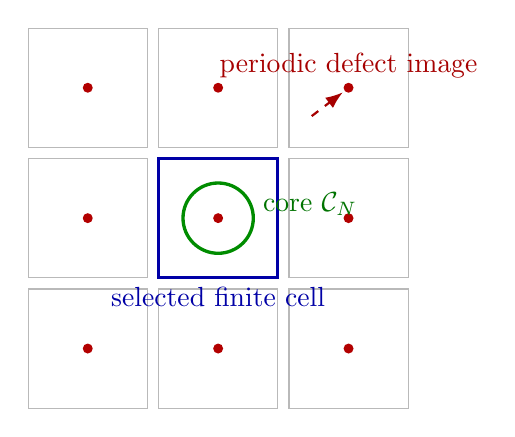
\begin{tikzpicture}[scale=0.72]
    \foreach \ix in {-1,0,1} {
      \foreach \iy in {-1,0,1} {
        \draw[gray!55] (2.3*\ix-1.05,2.3*\iy-1.05)
          rectangle (2.3*\ix+1.05,2.3*\iy+1.05);
        \fill[red!70!black] (2.3*\ix,2.3*\iy) circle (2.5pt);
      }
    }
    \draw[blue!65!black,very thick] (-1.05,-1.05) rectangle (1.05,1.05);
    \draw[green!55!black,very thick] (0,0) circle (0.62);
    \node[green!45!black,right] at (0.62,0.25) {core $\mathcal C_N$};
    \node[blue!65!black,below] at (0,-1.05) {selected finite cell};
    \node[red!65!black,above] at (2.3,2.3) {periodic defect image};
    \draw[protocolarrow,dashed,red!65!black] (1.65,1.8) -- (2.2,2.22);
  \end{tikzpicture}
  \caption{A finite periodic defect calculation represents an array of defect images.
  The isolated-defect-like limit is diagnosed by localized core weight, small exterior
  diagnostics, and diminishing twist dispersion as image separation increases.}
  \label{fig:periodic-defect-images}
\end{figure}

\subsection{Spectral and state diagnostics}

Let $E_{\mathrm{edge}}^{(N,\boldsymbol\phi)}$ be the declared parent host edge and let
$E_a^{(N,\boldsymbol\phi)}$ be a matched defect eigenvalue.  The binding energy and
below-edge count are
\begin{align}
  E_{b,a}^{(N,\boldsymbol\phi)}
  &=E_{\mathrm{edge}}^{(N,\boldsymbol\phi)}
    -E_a^{(N,\boldsymbol\phi)},\\
  n_{<}^{(N,\boldsymbol\phi)}
  &=\#\left\{a:
    E_a^{(N,\boldsymbol\phi)}
    <E_{\mathrm{edge}}^{(N,\boldsymbol\phi)}-\tau_b
  \right\}.
\end{align}
For a matched branch over the frozen twist mesh $\Phi$,
\begin{align}
  \overline E_N&=\frac{1}{|\Phi|}
    \sum_{\boldsymbol\phi\in\Phi}E_N(\boldsymbol\phi),\\
  W_N&=\max_{\boldsymbol\phi\in\Phi}E_N(\boldsymbol\phi)
      -\min_{\boldsymbol\phi\in\Phi}E_N(\boldsymbol\phi).
  \label{eq:defect-band-width}
\end{align}
The normalized image-coupling diagnostic may be reported as
\begin{equation}
  \omega_N=\frac{W_N}{B_N},
  \qquad
  B_N=E_{\max}^{\mathrm{parent}}-E_{\min}^{\mathrm{parent}},
  \label{eq:normalized-band-width}
\end{equation}
provided $B_N>0$.  No acceptance threshold for $\omega_N$ has yet been adopted.

For a normalized state $\psi$, define
\begin{align}
  p_C(\psi)&=\langle\psi|P_C|\psi\rangle,\\
  \operatorname{IPR}(\psi)&=\sum_{\mathbf n}|\psi_{\mathbf n}|^4,\\
  \bar x&=\sum_{\mathbf n}d_x(\mathbf n)|\psi_{\mathbf n}|^2,
  &\bar y&=\sum_{\mathbf n}d_y(\mathbf n)|\psi_{\mathbf n}|^2,\\
  r_x&=\sqrt{\sum_{\mathbf n}(d_x(\mathbf n)-\bar x)^2
                 |\psi_{\mathbf n}|^2},
  &r_y&=\sqrt{\sum_{\mathbf n}(d_y(\mathbf n)-\bar y)^2
                 |\psi_{\mathbf n}|^2},\\
  Q&=\frac{r_x^2-r_y^2}{r_x^2+r_y^2}.
  \label{eq:state-localization-diagnostics}
\end{align}
A radius-to-boundary separation diagnostic is
\begin{equation}
  \rho_N=\max\!\left(\frac{2r_x}{N_x},\frac{2r_y}{N_y}\right).
  \label{eq:radius-boundary-ratio}
\end{equation}
No acceptance threshold for $\rho_N$ has yet been adopted.

The eigenpair residual is
\begin{equation}
  r_{\mathrm{eig}}=\lVert H\psi-E\psi\rVert_2.
\end{equation}
For equal-rank orthonormal cluster bases $V$ and $W$, let
\begin{equation}
  \sigma_j=\sigma_j(V^{\dagger}W),
  \qquad
  \theta_j=\arccos\sigma_j.
\end{equation}
The projectors and overlap diagnostics are
\begin{align}
  P_V&=VV^{\dagger},&P_W&=WW^{\dagger},\\
  d_P&=\lVert P_V-P_W\rVert_F,
  &\sigma_{\min}&=\min_j\sigma_j.
  \label{eq:projector-diagnostics}
\end{align}
Individual vectors inside a degenerate cluster are not compared.

\subsection{Adjacent-size stability and perturbation strength}

Let $\mathbf d_N$ be the compatible local defect-coefficient record reconstructed at
size $N$.  For adjacent unaliased sizes $N<N'$, the prospective operator change is
\begin{equation}
  \delta_{\Delta}(N,N')
  =\frac{\lVert\mathbf d_{N'}-\mathbf d_N\rVert_2}
  {\max(\lVert\mathbf d_N\rVert_2,\epsilon_{\mathrm{norm}})}.
  \label{eq:adjacent-operator-change}
\end{equation}
An energy diagnostic $E$ is compared through
\begin{equation}
  \delta_E(N,N')
  =\frac{|E_{N'}-E_N|}{B_{N'}},
  \label{eq:adjacent-energy-change}
\end{equation}
while centers and radii retain absolute changes in lattice cells.  The normalization
floor $\epsilon_{\mathrm{norm}}$ must be adopted before execution; a zero or undeclared
denominator cannot be repaired after seeing results.

Spatial isolation is distinct from perturbation strength.  If a weak-perturbation
summary is requested, the preferred intensive quantity is
\begin{equation}
  \eta_N=\frac{\lVert\Delta_N\rVert_2}{B_N},
  \label{eq:weakness-ratio}
\end{equation}
not an extensive full-matrix Frobenius ratio whose denominator grows with cell area.
No threshold for $\eta_N$ is part of the current size-selection policy.

\section{Named research workstreams}

The maintained names below replace lettered names.  The legacy labels are retained only
as provenance crosswalks to the removed campaign.

\subsection{Folding and Null-Alignment Controls}
\noindent\textit{Historical provenance label: Stage A.}
Null extraction, finite folding, seam sign, and represented compatibility.  The
authored null/folding core is calculated and independently reconstructed; the seam
oracle, structured stops, and complete provenance contracts remain to be extracted.

\subsection{Onsite Extraction and Covariance Controls}
\noindent\textit{Historical provenance label: Stage B.}
Scalar onsite extraction, exact $D_4$ covariance, known-map controls, blind-map
ambiguity, representation routes, and schedule-order falsification.  This remains a
historical design donor and is not active or executable.

\subsection{Defect-Model Discrimination}
\noindent\textit{Historical provenance label: Stage C.}
Directional nearest-neighbour and finite-range nonlocal model classes with explicit
gauge-route reconciliation.  Historical authored-toy and accepted-parent donors exist,
but maintained contracts are not yet fully extracted.

\subsection{Finite-Domain Sensitivity}
\noindent\textit{Historical provenance label: Stage D.}
Separate area, fixed-area shape, orientation, and boundary-phase channels.  The exact
case inventory is retained as an unexecuted plan; operator production remains blocked.

\subsection{Composite-Subspace Extension}
\noindent\textit{Historical provenance label: Stage E.}
Coupled-parent and composite-subspace degeneracy controls.  This requires a separate
revision and has no active implementation or authority.

A later workstream is not activated merely because an earlier workstream passes.  Each
requires maintained typed contracts, active tests, independent verification, reviewed
inputs, and separate execution authority where applicable.

\begin{figure}[htbp]
  \centering
  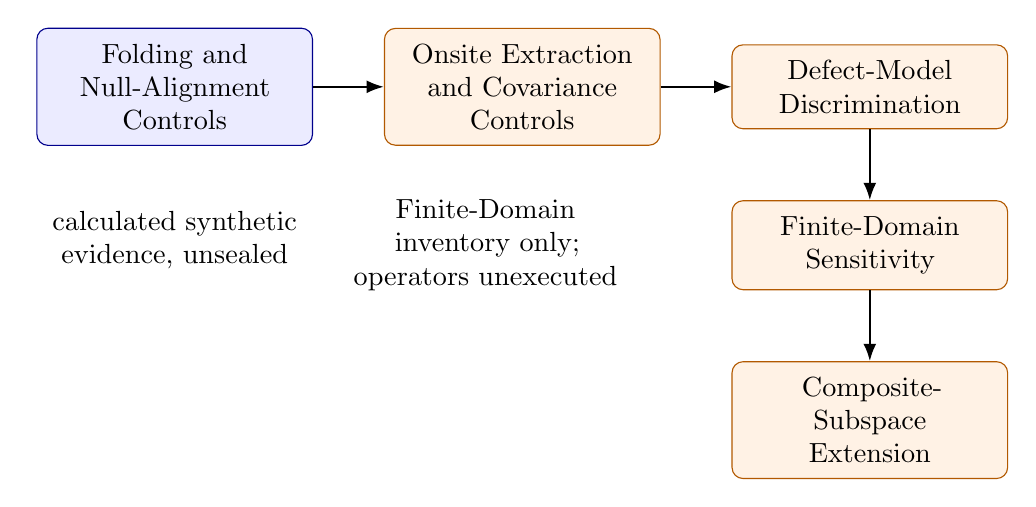
\begin{tikzpicture}[node distance=9mm and 9mm]
    \node[evidencebox] (fold) {Folding and\\Null-Alignment\\Controls};
    \node[plannedbox,right=of fold] (onsite) {Onsite Extraction\\and Covariance\\Controls};
    \node[plannedbox,right=of onsite] (model) {Defect-Model\\Discrimination};
    \node[plannedbox,below=of model] (finite) {Finite-Domain\\Sensitivity};
    \node[plannedbox,below=of finite] (composite) {Composite-Subspace\\Extension};
    \draw[protocolarrow] (fold) -- (onsite);
    \draw[protocolarrow] (onsite) -- (model);
    \draw[protocolarrow] (model) -- (finite);
    \draw[protocolarrow] (finite) -- (composite);
    \node[below=7mm of fold,align=center,text width=35mm]
      {calculated synthetic\\evidence, unsealed};
    \node[left=10mm of finite,align=center,text width=40mm]
      {Finite-Domain inventory only;\\operators unexecuted};
  \end{tikzpicture}
  \caption{Workstream gates.  Passing or retaining one workstream does not activate the
  next.  Only the folding/null core currently contains calculated synthetic evidence.}
  \label{fig:workstream-gates}
\end{figure}

\section{Folding and Null-Alignment Controls}

\subsection{Authored parent and attack}

The active parent is the immutable scalar hopping model
\path{authored-folding-null-parent} in basis \path{scalar-cell-basis}.  Its nonzero
coefficients are
\begin{center}
\begin{tabular}{cc}
\toprule
\textbf{Displacement $\mathbf R$} & \textbf{$h_{\mathbf R}$} \\
\midrule
$(0,0)$ & $0.20$ \\
$(1,0)$ and $(-1,0)$ & $-0.10$ \\
$(0,1)$ and $(0,-1)$ & $-0.08$ \\
\bottomrule
\end{tabular}
\end{center}
The coefficients are dimensionless and exactly Hermitian.  This parent is a software
and numerical-verification object, not the historical accepted periodic parent.

The null attack applies translation by $(1,1)$ cells, site-phase steps
$(0.137,-0.191)$ radians, and scalar energy-reference shift $c=0.137$.  With declared
unitary $G$,
\begin{align}
  \widetilde H &= GHG^\dagger+cI, \\
  \Delta_{\mathrm{rec}} &= G^\dagger(\widetilde H-cI)G-H.
\end{align}
This known-map null control does not establish that $G$ or $c$ can be inferred blindly
from a homogeneous parent.

\begin{figure}[htbp]
  \centering
  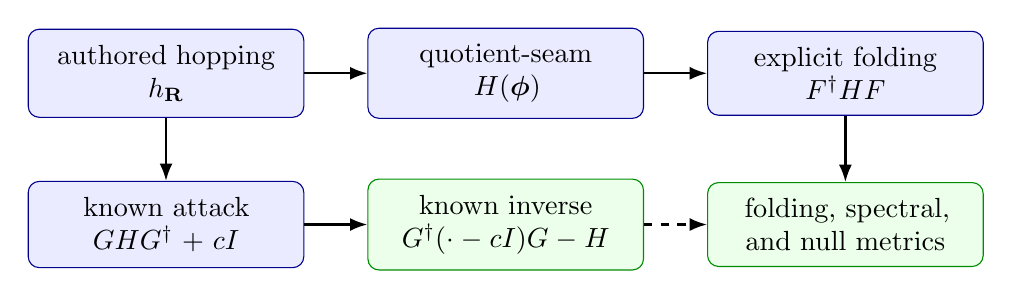
\begin{tikzpicture}[node distance=8mm and 8mm]
    \node[evidencebox] (terms) {authored hopping\\$h_{\mathbf R}$};
    \node[evidencebox,right=of terms] (seam) {quotient-seam\\$H(\boldsymbol\phi)$};
    \node[evidencebox,right=of seam] (fold) {explicit folding\\$F^{\dagger}HF$};
    \node[evidencebox,below=of terms] (attack) {known attack\\$GHG^{\dagger}+cI$};
    \node[verifybox,right=of attack] (inverse) {known inverse\\$G^{\dagger}(\cdot-cI)G-H$};
    \node[verifybox,right=of inverse] (metrics) {folding, spectral,\\and null metrics};
    \draw[protocolarrow] (terms) -- (seam);
    \draw[protocolarrow] (seam) -- (fold);
    \draw[protocolarrow] (terms) -- (attack);
    \draw[protocolarrow] (attack) -- (inverse);
    \draw[protocolarrow] (fold) -- (metrics);
    \draw[protocolarrow,dashed] (inverse) -- (metrics);
  \end{tikzpicture}
  \caption{Active authored folding/null calculation.  Folding and known-inverse null
  recovery are separate diagnostics of the same represented parent matrix.}
  \label{fig:active-folding-null-schematic}
\end{figure}

\subsection{Frozen case inventory}

The control suite uses shapes $6\times6$ and $8\times8$ at twists
\begin{equation}
  (0,0),\quad(0.37,-0.23),\quad(0.5,0),\quad(0,0.5).
\end{equation}
Each of the eight cases retains folding unitarity, represented-parent Hermiticity,
folded off-diagonal magnitude, primitive-energy reconstruction, folded-spectrum,
null-transform unitarity, recovered maximum-entry, and recovered Frobenius defects.
The prospective algebraic and folding-unitarity tolerances are both $10^{-11}$.  The
retained result passes and independent reconstruction agrees with a maximum metric
difference of $3.47274002286861\times10^{-16}$.

\begin{figure}[htbp]
  \centering
  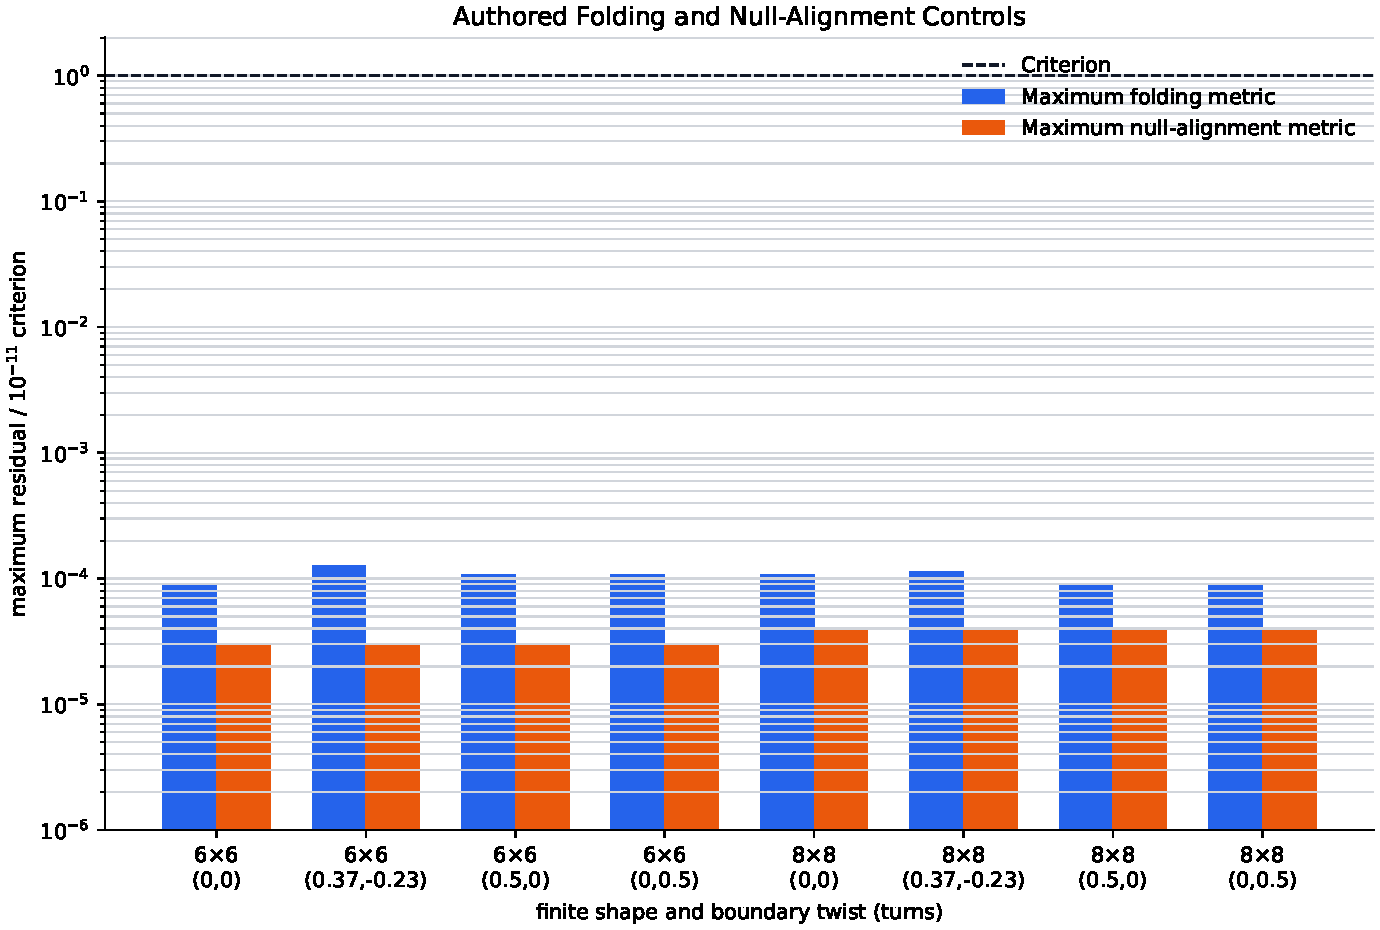
\includegraphics[width=\textwidth]{folding-null-residuals.pdf}
  \caption{Maximum retained folding and null-alignment metrics for each authored
  shape/twist case, normalized by the prospective $10^{-11}$ criterion.  The plot is
  dimensionless synthetic numerical evidence only; the distance below the criterion
  is not a material uncertainty or a scientific-validation margin.}
  \label{fig:folding-null-residuals}
\end{figure}

\subsection{Pending exact controls}

The seam oracle uses a one-dimensional size-six seam at twist $0.37$ turns and checks
phase $1$ for a noncrossing displacement, $\exp(2\pi i\,0.37)$ for source 5 and
displacement $+1$, and $\exp(-2\pi i\,0.37)$ for source 0 and displacement $-1$.

\begin{center}
\small
\begin{tabularx}{\textwidth}{>{\raggedright\arraybackslash}p{0.22\textwidth}YY}
\toprule
\textbf{Control} & \textbf{Candidate mismatch} & \textbf{Required stop} \\
\midrule
Incorrect geometry & $(6,6)$ pristine versus $(8,6)$ candidate & \path{DEFECT_2D.GEOMETRY_MISMATCH} \\
Incorrect boundary phase & $(0,0)$ pristine versus $(0.5,0)$ candidate twist & \path{DEFECT_2D.BOUNDARY_PHASE_MISMATCH} \\
Lost site correspondence & Candidate site map unknown & \path{DEFECT_2D.SITE_MAP_UNRESOLVED} \\
Unknown energy reference & Candidate energy relation unknown & \path{DEFECT_2D.ENERGY_REFERENCE_UNKNOWN} \\
\bottomrule
\end{tabularx}
\end{center}
The producer and verifier derive these stops from metadata; they do not copy expected
issue codes into observed results.

\section{Successor defect and model controls}

The frozen synthetic defect sequence is null; scalar onsite strength $-0.25$ at $(0,0)$;
the same onsite defect at $(1,2)$ and its complete $D_4$ orbit; directional
nearest-neighbour changes $+0.04$ along positive $x$ and $-0.03$ along positive $y$; a
diagonal finite-range change $+0.025$ at displacement $(1,1)$; and, only in the future
composite branch, a rank-three onsite block.  Every bond change includes its Hermitian
reverse.

The nested scalar model hierarchy is:
\begin{enumerate}[leftmargin=*]
  \item point scalar onsite;
  \item finite-support diagonal onsite;
  \item onsite plus isotropic nearest neighbour;
  \item onsite plus directional nearest neighbour; and
  \item finite-range nonlocal radius two.
\end{enumerate}
Projection uses the represented Frobenius inner product.  The selected class is the
first frozen class satisfying every applicable criterion.  A favorable eigenvalue or
one favorable route cannot select a class.

\subsection{Authored Defect-Model Discrimination controls}

The authored control suite preserves an $8\times8$ scalar space and twists $(0,0)$ and
$(0.37,-0.23)$.  Route A uses the centered uniform-link gauge and Route B the
quotient-seam gauge.  An explicit site-diagonal bridge relates them; they are not
independent estimates.  Each case is evaluated in A-then-B and B-then-A schedules in
fresh processes.

The represented defect must be Hermitian within $10^{-12}$, and the first accepted
model class must have maximum-entry and Frobenius residuals no greater than $10^{-12}$.
Independent reconstruction is limited by $10^{-11}$.  Frozen adverse controls require
an isotropic fit to the directional defect and a directional fit to the diagonal defect
to retain Frobenius residual at least $0.03$; omission of a Hermitian reverse to produce
Hermiticity defect at least $0.03$; and an unbridged generic-twist route comparison to
differ by at least $0.01$ in maximum entry.  These are discrimination floors, not
physical uncertainty estimates.

\section{Alignment and extraction policy}

A planted control is defined in a canonical frame,
\begin{equation}
  H_{\mathrm{def}}=H_{\mathrm{pris}}+\Delta_{\mathrm{plant}}.
\end{equation}
A candidate may include a declared lattice translation, point-group operation, site
phases, orbital action where applicable, and scalar energy shift.  Extraction
\begin{equation}
  \Delta_{\mathrm{rec}}=
  G^\dagger(\widetilde H_{\mathrm{def}}-cI)G-H_{\mathrm{pris}}
\end{equation}
is permitted only after compatibility is established.

Known-map and blind-map routes are distinct experiments.  The known-map route receives
the authored transformation.  A blind route does not read the plant, known map, or
known-map residual.  If a homogeneous parent leaves translations or point-group actions
tied, the route returns an ambiguity set and
\path{DEFECT_2D.SITE_MAP_UNRESOLVED}; it does not select a map using the plant.
Pre-alignment subtraction and omission of the energy correction are negative controls,
not defect estimates.

The inactive successor attack preserves translation $(2,3)$, point-group operation
\path{reflection_x_after_quarter_turn}, site-phase steps $(0.137,-0.191)$ radians, and
energy shift $0.137$.  The blind search covers all periodic translations and all allowed
point-group operations.  For each candidate map $G_{M,\mathbf t}$, its frozen objective
is
\begin{equation}
  J(M,\mathbf t)
  =\left\lVert
    \operatorname{offdiag}\!\left(
      G_{M,\mathbf t}^{\dagger}\widetilde H_{\mathrm{def}}G_{M,\mathbf t}
      -H_{\mathrm{pris}}
    \right)
  \right\rVert_F.
\end{equation}
After phase recovery anchored at $(0,0)$, the scalar shift diagnostic is
\begin{equation}
  \widehat c
  =\operatorname{median}_{\mathbf n}
    \operatorname{Re}\left[
      \left(
        G^{\dagger}\widetilde H_{\mathrm{def}}G-H_{\mathrm{pris}}
      \right)_{\mathbf n\mathbf n}
    \right].
\end{equation}
The search stops when candidates tie within $10^{-10}$ or the nonzero parent hopping
graph is disconnected.

\subsection{Onsite-extraction multi-route boundary}

The superseded single-route design is not reactivated.  Route A constructs the
$8\times8$ operator directly in a centered uniform-link gauge from unreduced lift
$\widetilde\phi\in[-1/2,1/2)^2$.  Route B constructs directly in the reduced seam gauge.
The diagonal bridge
\begin{equation}
  D(\widetilde\phi)|x\rangle=
  \exp\!\left[2\pi i\left(
    \frac{x_1\widetilde\phi_1}{N_1}+
    \frac{x_2\widetilde\phi_2}{N_2}
  \right)\right]|x\rangle
\end{equation}
must satisfy
\begin{equation}
  H_B(\widetilde\phi\bmod1)=
  D(\widetilde\phi)H_A(\widetilde\phi)D(\widetilde\phi)^\dagger.
\end{equation}
Neither route is obtained by transforming the other.  The bridge is an equivalence
check, not a third estimate; routes are never averaged, ranked, or allowed to vote.

\begin{figure}[htbp]
  \centering
  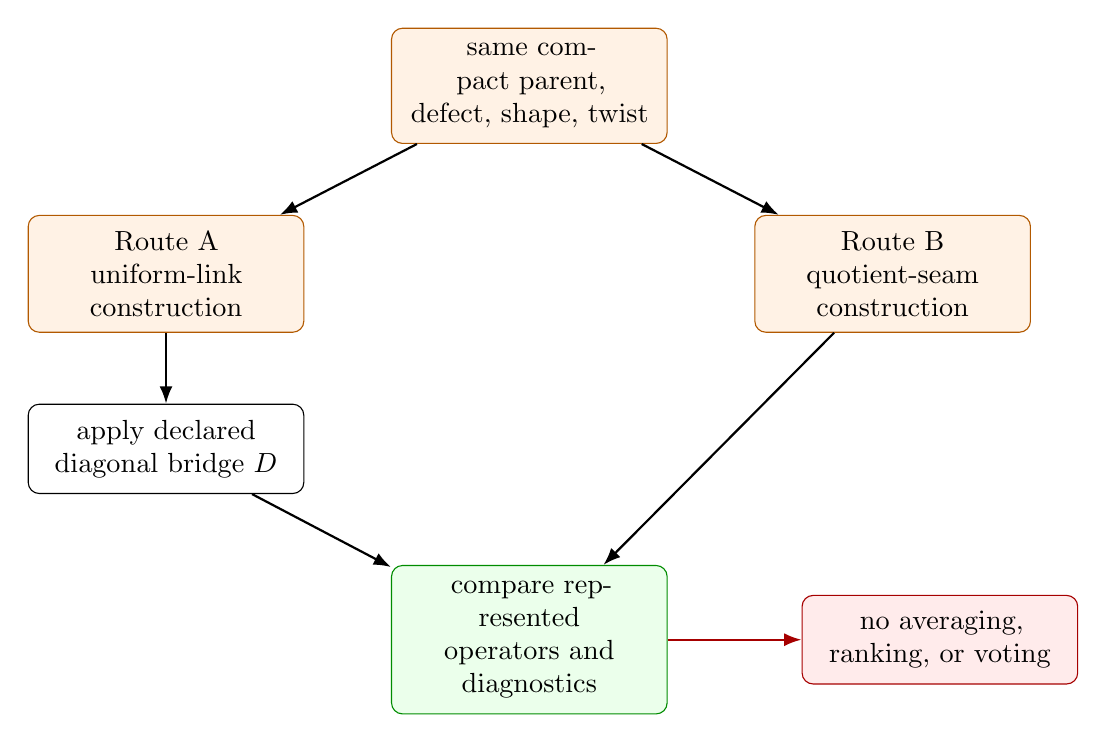
\begin{tikzpicture}[node distance=9mm and 11mm]
    \node[plannedbox] (source) {same compact parent,\\defect, shape, twist};
    \node[plannedbox,below left=of source] (routea)
      {Route A\\uniform-link construction};
    \node[plannedbox,below right=of source] (routeb)
      {Route B\\quotient-seam construction};
    \node[protocolbox,below=of routea] (bridge)
      {apply declared\\diagonal bridge $D$};
    \node[verifybox,below right=of bridge] (compare)
      {compare represented\\operators and diagnostics};
    \draw[protocolarrow] (source) -- (routea);
    \draw[protocolarrow] (source) -- (routeb);
    \draw[protocolarrow] (routea) -- (bridge);
    \draw[protocolarrow] (bridge) -- (compare);
    \draw[protocolarrow] (routeb) -- (compare);
    \node[stopbox,right=of compare,xshift=6mm] (novote)
      {no averaging,\\ranking, or voting};
    \draw[protocolarrow,red!65!black] (compare) -- (novote);
  \end{tikzpicture}
  \caption{Prospective multi-route gauge check.  Both routes construct the operator
  directly.  The bridge reconciles gauges before comparison and does not create a
  third estimate.}
  \label{fig:multi-route-gauge-schematic}
\end{figure}

The off-axis site $(1,2)$ owns orbit
\begin{equation}
  (1,2),(6,1),(7,6),(2,7),(1,6),(7,2),(2,1),(6,7).
\end{equation}
Each route has 18 known-map cases.  A Gamma blind search retains 512 tied
point-group/translation candidates; a generic-twist search retains 64 tied translations.
The shift diagnostic is the median real aligned diagonal difference, not the trace mean.
Across two fresh-process schedules, the frozen inventory has 72 route-local known-map
evaluations, 36 cross-route records, and 2,304 blind candidate evaluations.  A
disconnected hopping graph stops with
\path{DEFECT_2D.PHASE_GRAPH_DISCONNECTED}.

\section{Symmetry and orientation policy}

For the isotropic scalar parent, define the integer generators
\begin{equation}
  R=\begin{pmatrix}0&-1\\1&0\end{pmatrix},
  \qquad
  S=\begin{pmatrix}1&0\\0&-1\end{pmatrix}.
\end{equation}
The frozen group is
\begin{equation}
  D_4=\{I,R,R^2,R^3,S,R^2S,RS,R^3S\},
\end{equation}
ordered as identity, quarter turn, half turn, three-quarter turn, reflection in $x$,
reflection in $y$, diagonal reflection, and antidiagonal reflection.  Each operation
acts through the exact integer coordinate map followed by periodic reduction.  At
nonzero twist,
\begin{equation}
  \boldsymbol\phi\mapsto M\boldsymbol\phi\pmod 1.
\end{equation}
Covariance compares the transformed fiber.  Holding a generic twist fixed under a
quarter turn is a required negative control.

For the anisotropic parent, self-symmetry is the declared $D_2$ subgroup.  An axis swap
maps the source parent to the separately identified parent with exchanged $x$ and $y$
coefficients.  The same-parent orientation contrast, which has no zero expectation, and
source-to-swapped-parent covariance, which is algebraic, remain separate.

\begin{figure}[htbp]
  \centering
  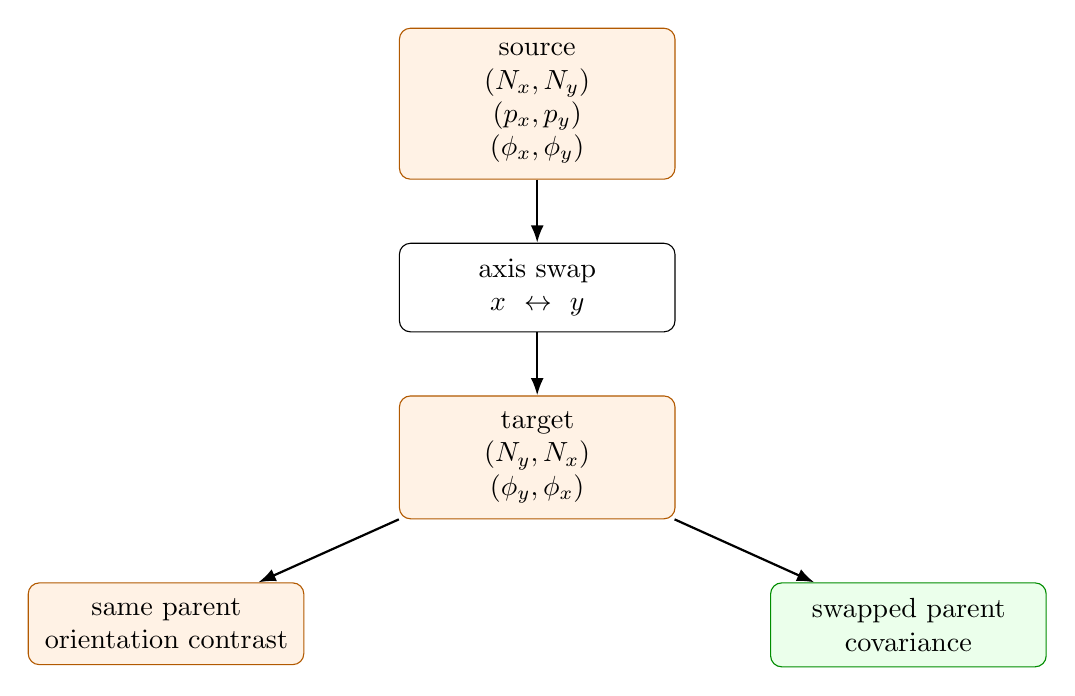
\begin{tikzpicture}[node distance=8mm and 12mm]
    \node[plannedbox] (source)
      {source\\$(N_x,N_y)$\\$(p_x,p_y)$\\$(\phi_x,\phi_y)$};
    \node[protocolbox,below=of source] (swap)
      {axis swap\\$x\leftrightarrow y$};
    \node[plannedbox,below=of swap] (target)
      {target\\$(N_y,N_x)$\\$(\phi_y,\phi_x)$};
    \node[plannedbox,below left=of target] (same)
      {same parent\\orientation contrast};
    \node[verifybox,below right=of target] (cov)
      {swapped parent\\covariance};
    \draw[protocolarrow] (source) -- (swap);
    \draw[protocolarrow] (swap) -- (target);
    \draw[protocolarrow] (target) -- (same);
    \draw[protocolarrow] (target) -- (cov);
  \end{tikzpicture}
  \caption{Orientation policy.  Geometry, defect support, and twist transform together.
  Same-parent contrast and swapped-parent covariance answer different questions.}
  \label{fig:orientation-schematic}
\end{figure}

\section{Composite-Subspace Extension}

This workstream remains inactive and requires a revision before implementation.  The
historical rank-three onsite block is
\begin{equation}
  \begin{pmatrix}
  -0.30 & 0.04 & -0.02\\
  0.04 & -0.16 & 0.03\\
  -0.02 & 0.03 & -0.08
  \end{pmatrix}.
\end{equation}
The frozen orbital attack uses permutation $(2,0,1)$, rotations in pairs $(0,1)$ and
$(1,2)$ by $0.31$ and $-0.27$ radians, and orbital phases
$(0.11,-0.23,0.37)$ radians.  If $R_{ab}(\theta)$ denotes the identity with the
$(a,b)$ block
\begin{equation}
  \begin{pmatrix}
    \cos\theta & -\sin\theta\\
    \sin\theta & \cos\theta
  \end{pmatrix},
\end{equation}
and $P_{(2,0,1)}$ is the declared permutation, the frozen orbital action is
\begin{equation}
  U_{\mathrm{orb}}
  =\operatorname{diag}\!\left(e^{0.11i},e^{-0.23i},e^{0.37i}\right)
   R_{12}(-0.27)R_{01}(0.31)P_{(2,0,1)}.
\end{equation}
The represented action on the composite finite space is
$G_{\mathrm{site}}\otimes U_{\mathrm{orb}}$.  The coupled scalar-parent control uses
$\lambda_{xy}=0.15$ rather than $\lambda_{xy}=0$.  No current contract or retained
result activates these selections.

\section{Finite-Domain Sensitivity}

The retained version-2 planning definition fixes four nonpooled channels and adds the
previously omitted $1\times1$ through $5\times5$ square cells as explicit small-cell
periodic-aliasing controls.  The version-1 inventory remains retained and is not
rewritten.

\subsection{Area}
The ordered square inventory is
\begin{equation}
  (1,1),\ (2,2),\ (3,3),\ (4,4),\ (5,5),\ (6,6),\ (8,8),\
  (10,10),\ (12,12),\ (16,16).
\end{equation}
The $1\times1$ through $4\times4$ quotients alias the radius-two defect support with
periodic images.  The $5\times5$ through $8\times8$ cells separate that radius-two core
but can still alias distinct displacements in the retained parent support
$R_x^2+R_y^2\leq18$.  The selected $10\times10$ and larger cells are unaliased for that
retained displacement inventory.  These classifications follow from integer quotient
geometry; they are not operator results.

Area is the only ordered finite-size sequence, but small-cell aliasing controls are not
interpreted as isolated-defect or convergence evidence.  The final $12\times12$ to
$16\times16$ comparison remains the only prospective final-step reporting comparison.
Failed or nonmonotone changes remain reported.

\begin{figure}[htbp]
  \centering
  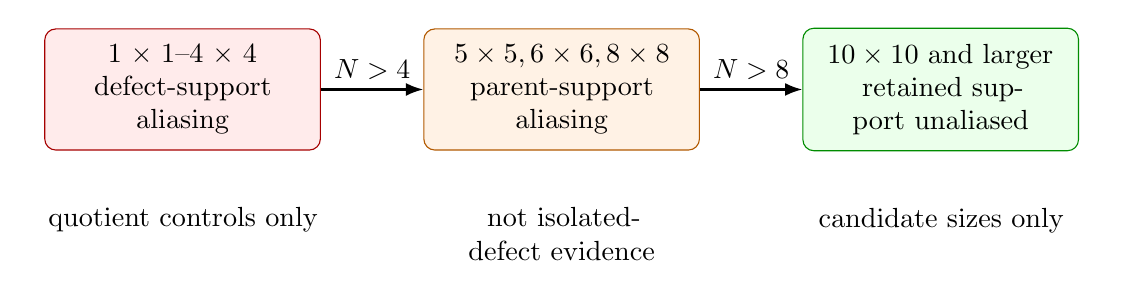
\begin{tikzpicture}[node distance=8mm and 13mm]
    \node[stopbox] (small) {$1\times1$--$4\times4$\\defect-support aliasing};
    \node[plannedbox,right=of small] (middle)
      {$5\times5,6\times6,8\times8$\\parent-support aliasing};
    \node[verifybox,right=of middle] (large)
      {$10\times10$ and larger\\retained support unaliased};
    \draw[protocolarrow] (small) -- node[above] {$N>4$} (middle);
    \draw[protocolarrow] (middle) -- node[above] {$N>8$} (large);
    \node[below=6mm of small,align=center,text width=37mm]
      {quotient controls only};
    \node[below=6mm of middle,align=center,text width=39mm]
      {not isolated-defect evidence};
    \node[below=6mm of large,align=center,text width=38mm]
      {candidate sizes only};
  \end{tikzpicture}
  \caption{Finite-square support regimes implied by
  Eq.~\eqref{eq:support-size-condition}.  ``Unaliased'' is a structural prerequisite,
  not proof of negligible periodic-image coupling.}
  \label{fig:aliasing-regimes}
\end{figure}

\subsection{Shape}
The fixed-area-144 geometries are
\begin{equation}
  (8,18),\ (9,16),\ (12,12),\ (16,9),\ (18,8).
\end{equation}
Shape is a contrast at fixed cell count, not a convergence sequence.  Matrices on
different geometries are not directly subtracted.

\subsection{Orientation}
The pairs are
\begin{equation}
  (8,18)\leftrightarrow(18,8),\qquad
  (9,16)\leftrightarrow(16,9).
\end{equation}
Coordinates, defect displacements, and twists exchange $x$ and $y$.  Each record
requires a source evaluation, same-parent rotated-target evaluation, and swapped-parent
rotated-target evaluation.

\subsection{Boundary phase}
Every applicable geometry uses
\begin{equation}
  (\phi_x,\phi_y)=\left(\frac{m}{9},\frac{n}{9}\right),
  \qquad m,n\in\{0,\ldots,8\},
\end{equation}
with first component outer and second inner.  No favorable twist is selected, omitted,
or reweighted after observing results.

\subsection{Smallest isolated-defect-like cell objective}

The primary finite-size objective is to identify the smallest square cell that behaves
as an isolated localized defect perturbation.  This is distinct from asking whether the
defect is weak.  Spatial isolation concerns the support of the extracted operator and
the coupling between periodic defect images.  Weakness concerns a separately normalized
operator magnitude such as $\lVert\Delta_N\rVert/\lVert H_N\rVert$.  A spatially
localized defect may be strong, and a small-norm perturbation may be spatially extended.
No weak-perturbation conclusion is required for size selection.

A finite periodic cell represents a periodic array of defects.  For a matched
nondegenerate defect state, its twist dispersion is summarized by
\begin{equation}
  W_N = \max_{\boldsymbol\phi} E_N(\boldsymbol\phi)
      - \min_{\boldsymbol\phi} E_N(\boldsymbol\phi).
\end{equation}
For a degenerate or multistate defect cluster, the protocol uses transported projectors
and cluster spectral ranges rather than independently ordered vectors.  Decreasing
$W_N$ is evidence of reduced periodic-image coupling, but monotonic decrease is an
expected trend rather than a verification oracle.

The size assessment retains, without pooling:
\begin{enumerate}[leftmargin=*]
  \item compatibility, alignment, and independent-reconstruction status;
  \item radius-two core, exterior, and core--exterior operator diagnostics;
  \item twist-resolved defect-band center and width;
  \item host-edge-referenced binding energy and below-edge state count;
  \item projector fidelity, core probability, inverse participation ratio, and separate
    $x/y$ RMS radii; and
  \item changes in the compatible local coefficient record and scalar diagnostics
    between adjacent support-unaliased sizes.
\end{enumerate}

The $1\times1$ through $8\times8$ cells are aliasing controls and cannot support an
isolated-defect claim.  The $10\times10$, $12\times12$, and $16\times16$ cells are the
current support-unaliased candidates.  A selected size must be the smaller member of an
adjacent candidate pair that satisfies all prospectively adopted absolute-isolation and
adjacent-size stability criteria.  Therefore the current candidate comparisons are
$10\times10\rightarrow12\times12$ and
$12\times12\rightarrow16\times16$.  If neither pair passes, no size is selected and a
larger-cell inventory is required; $16\times16$ cannot be certified as the smallest
adequate size without a larger confirmation cell.

The current protocol has frozen final-step reporting criteria for operator, energy,
center, and radius changes, but it has not adopted absolute thresholds for defect-band
width, exterior weight, core probability, or radius-to-boundary separation.  Those
thresholds must be fixed in a versioned request before operator production.  Until then,
$10\times10$ is only the first structurally admissible candidate, not an accepted
supercell size.

\begin{figure}[htbp]
  \centering
  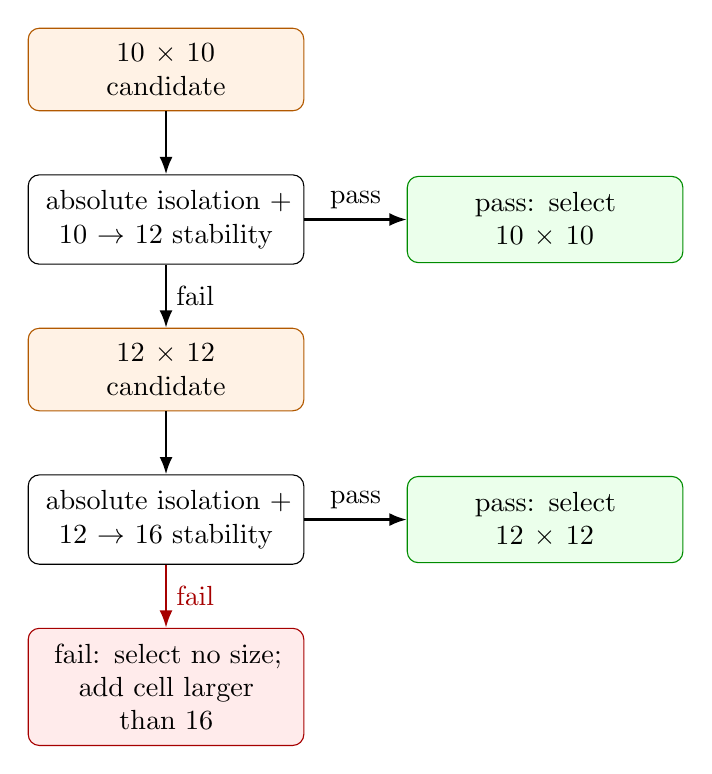
\begin{tikzpicture}[node distance=8mm and 13mm]
    \node[plannedbox] (n10) {$10\times10$\\candidate};
    \node[protocolbox,below=of n10] (c1012)
      {absolute isolation +\\$10\rightarrow12$ stability};
    \node[verifybox,right=of c1012] (select10)
      {pass: select\\$10\times10$};
    \node[plannedbox,below=of c1012] (n12) {$12\times12$\\candidate};
    \node[protocolbox,below=of n12] (c1216)
      {absolute isolation +\\$12\rightarrow16$ stability};
    \node[verifybox,right=of c1216] (select12)
      {pass: select\\$12\times12$};
    \node[stopbox,below=of c1216] (larger)
      {fail: select no size;\\add cell larger than $16$};
    \draw[protocolarrow] (n10) -- (c1012);
    \draw[protocolarrow] (c1012) -- node[above] {pass} (select10);
    \draw[protocolarrow] (c1012) -- node[right] {fail} (n12);
    \draw[protocolarrow] (n12) -- (c1216);
    \draw[protocolarrow] (c1216) -- node[above] {pass} (select12);
    \draw[protocolarrow,red!65!black] (c1216) -- node[right] {fail} (larger);
  \end{tikzpicture}
  \caption{Prospective smallest-size selection ladder.  The smaller member of a passing
  adjacent pair is selected.  The largest retained size cannot certify itself.}
  \label{fig:size-selection-ladder}
\end{figure}

The exact version-2 unexecuted inventory contains 2,268 unique isotropic cases, 324
orientation comparison records, 972 orientation operator evaluations, and 3,240
proposed operator evaluations.  Shared $12\times12$ isotropic cases belong to area and
shape channels and are evaluated once.  The exact accounting is
\begin{align}
  N_{\mathrm{iso}}&=14\times2\times81=2268,\\
  N_{\mathrm{orient,records}}&=2\times2\times81=324,\\
  N_{\mathrm{orient,eval}}&=3\times324=972,\\
  N_{\mathrm{total}}&=2268+972=3240.
\end{align}
The 810 additional isotropic cases are
$5\times2\times81=810$: five added square geometries times two defects times 81 twists.

\begin{figure}[htbp]
  \centering
  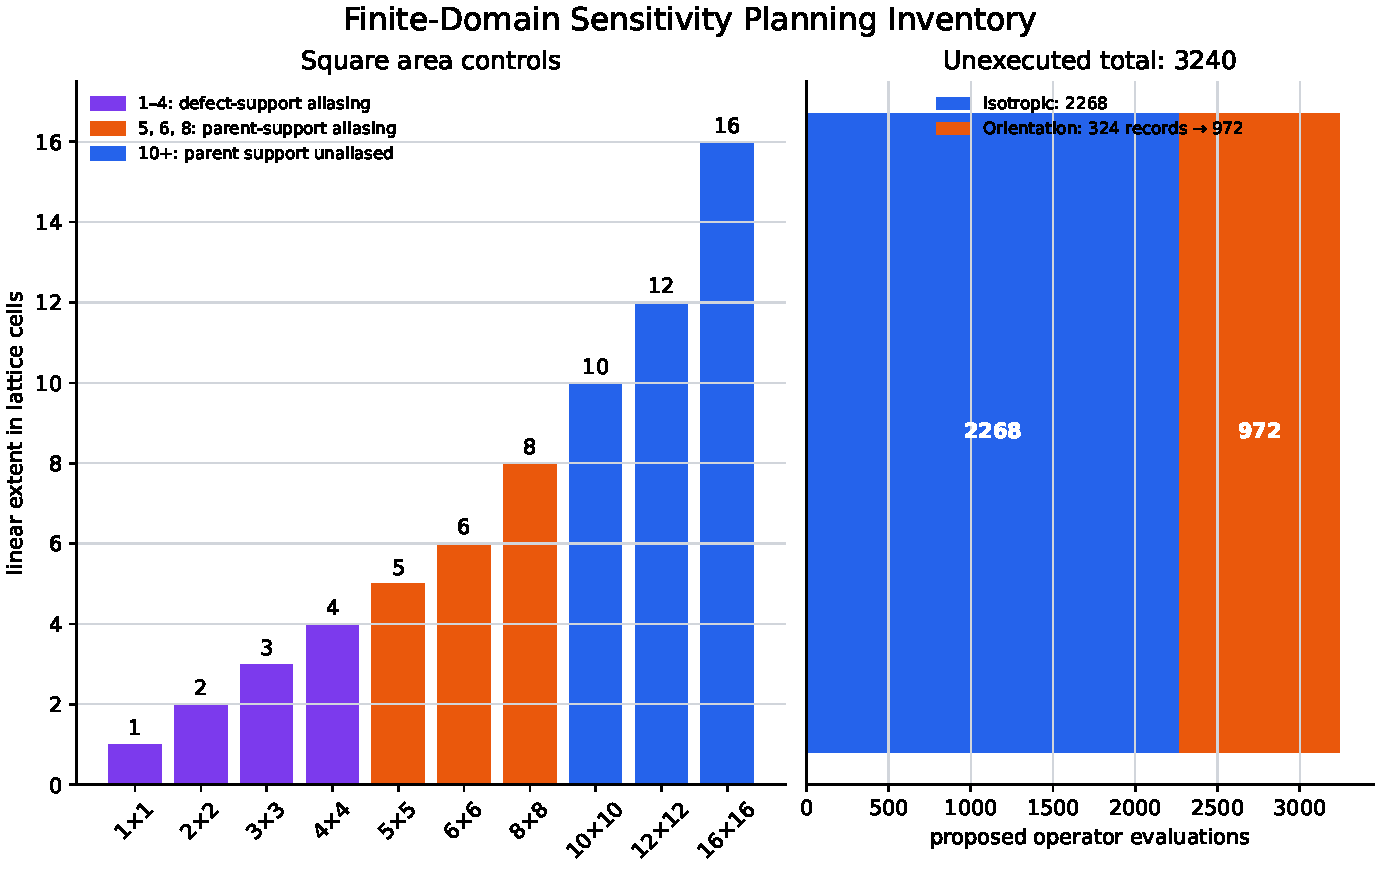
\includegraphics[width=\textwidth]{finite-domain-inventory.pdf}
  \caption{Retained version-2 Finite-Domain Sensitivity planning inventory, including
  $1\times1$ through $5\times5$ small-cell aliasing controls.  The 972 orientation
  evaluations are the three proposed operator evaluations attached to each of 324
  orientation-comparison records.  All 3,240 evaluations remain unexecuted; this figure
  is an inventory visualization, not a finite-domain scientific result.}
  \label{fig:finite-domain-inventory}
\end{figure}
\clearpage

\section{Recommended graph and figure program}

The human instruction \emph{recommendation authorized} authorizes the documented
recommendation in this section.  It does not authorize accepted-parent construction,
operator production, execution of the 3,240 proposed evaluations, external computation,
or relaxation of the parent-capability parity gate.

The recommended presentation is an atlas rather than one pooled dashboard.  Every
scientific graph retains defect identity, geometry, twist inventory, gauge route,
energy reference, and execution status.  The statuses below are:
\begin{itemize}[leftmargin=*]
  \item \textbf{retained}: already supported by retained calculated evidence;
  \item \textbf{planning}: constructible from the execution-free inventory and frozen
    support geometry without producing defect operators; and
  \item \textbf{blocked}: requires the future operator-producing campaign and its
    independent reconstruction.
\end{itemize}

\footnotesize
\begin{longtable}{@{}L{10mm}L{42mm}L{65mm}L{18mm}@{}}
\caption{Recommended complete graph program.}\label{tab:recommended-figures}\\
\toprule
\textbf{ID} & \textbf{Graph} & \textbf{Decision or diagnostic role} & \textbf{Status} \\
\midrule
\endfirsthead
\toprule
\textbf{ID} & \textbf{Graph} & \textbf{Decision or diagnostic role} & \textbf{Status} \\
\midrule
\endhead
P01 & Square-size and support-regime inventory & Separate defect-support aliasing,
parent-support aliasing, and support-unaliased candidates. & planning \\
P02 & Parent-displacement collision count versus $N$ & Count distinct support terms
that collapse into common quotient entries. & planning \\
P03 & Displacement-equivalence maps for $N=1,\ldots,8$ & Show exactly which primitive
displacements alias in each control cell. & planning \\
P04 & Radius-two defect support in every small quotient & Expose defect-image overlap
and bond collapse before operator interpretation. & planning \\
P05 & Complete $9\times9$ twist-mesh diagram & Make the no-cherry-picking boundary
phase inventory visible. & planning \\
P06 & Fixed-area shape and orientation gallery & Display area, shape, and axis-swap
comparisons without treating them as one sequence. & planning \\
P07 & Case-count and evaluation-accounting chart & Reconstruct the 2,268 isotropic,
324 orientation-record, 972 orientation-evaluation, and 3,240 total counts. & planning \\
V01 & Folding/null residuals by shape and twist & Retain the active synthetic numerical
control relative to its prospective criterion. & retained \\
V02 & Separate folding metric panels & Show unitarity, Hermiticity, off-diagonal,
primitive-energy, and spectral defects without a maximum-only summary. & retained \\
V03 & Exact seam-oracle phase diagram & Show noncrossing and positive/negative seam
crossings with their expected complex phases. & planning \\
V04 & Uniform-link to quotient-seam bridge residual & Test gauge equivalence for every
qualified parent and frozen perturbation identity. & retained \\
V05 & Production versus independent-reconstruction residual & Retain the aggregate
maximum independent metric difference separately from physical adequacy. & retained \\
V06 & Qualification runtime and memory observations & Retain measured calculation and
verification resources at the complete-inventory maximum dimension without fitting a
scaling law. & retained \\
I01 & Normalized defect-band width $\omega_N=W_N/B_N$ versus $N$ & Primary measure of
periodic-image coupling for support-unaliased candidates. & blocked \\
I02 & Absolute defect-band width $W_N$ versus $N$ & Preserve the dimensional energy
scale hidden by normalization. & blocked \\
I03 & Binding energy versus $N$ with complete twist envelope & Test size stability while
showing every twist rather than only a mean. & blocked \\
I04 & Binding-energy heatmap over $(\phi_x,\phi_y)$ for each size & Reveal anisotropic or
localized twist sensitivity and unfavorable fibers. & blocked \\
I05 & Near-edge spectrum versus twist & Expose defect-band formation, crossings,
cluster changes, and host-edge movement. & blocked \\
I06 & Below-edge state count over size and twist & Detect unstable bound-state
classification and retain no-bound-state cases. & blocked \\
I07 & Core, core--exterior, and exterior operator fractions & Establish whether the
extracted perturbation remains spatially local. & blocked \\
I08 & Core probability and inverse participation ratio versus $N$ & Characterize state
localization through complementary diagnostics. & blocked \\
I09 & $r_x$, $r_y$, $\rho_N$, and quadrupole anisotropy versus $N$ & Compare state size,
boundary separation, and directional distortion. & blocked \\
I10 & Real-space state-density maps by size and representative twist & Show defect-image
hybridization that scalar summaries can conceal. & blocked \\
I11 & Shell-resolved state probability and perturbation Frobenius weight & Separate
compact core behavior from extended tails. & blocked \\
I12 & Perturbation-strength--localization plane $(\eta_N,\rho_N)$ & Keep weak and
localized perturbation claims distinct. & blocked \\
D01 & Recovered local defect coefficients versus $N$ & Test whether the extracted local
operator stabilizes with size. & blocked \\
D02 & Per-coefficient changes for $10\to12$ and $12\to16$ & Prevent cancellation inside
a pooled operator norm. & blocked \\
D03 & Adjacent-size $\delta_{\Delta}$ and $\delta_E$ & Apply the declared operator and
energy stability definitions. & blocked \\
D04 & Changes in band center, width, core probability, IPR, and radii & Retain each
selection-relevant scalar diagnostic separately. & blocked \\
D05 & Candidate-pair criterion matrix & Display pass, failure, unavailable, and
structured-stop status for every criterion. & blocked \\
D06 & Populated smallest-size decision ladder & Select the smaller passing candidate or
record that no size was selected. & blocked \\
M01 & Residual versus nested model class & Show the first class satisfying every frozen
operator criterion. & blocked \\
M02 & Recovered versus planted coefficients & Verify amplitude and directional recovery
for authored controls. & blocked \\
M03 & Adverse-control residual panels & Retain isotropic-on-directional,
directional-on-diagonal, omitted-reverse, and unbridged-gauge failures. & blocked \\
M04 & Support and model-class confusion matrix & Expose systematic misclassification
rather than reporting only selected classes. & blocked \\
S01 & $D_4$ covariance residual by operation and twist & Test exact integer symmetry
maps and transformed fibers. & blocked \\
S02 & Same-parent orientation contrast and swapped-parent covariance & Keep physical
contrast separate from algebraic covariance. & blocked \\
S03 & Fixed-area shape dependence of every accepted scalar diagnostic & Report shape
sensitivity without calling it convergence. & blocked \\
C01 & Parent adjacent gaps and selected cluster ranks & Make degeneracy decisions and
rank changes explicit. & blocked \\
C02 & Principal angles, minimum singular overlap, and projector distance & Replace
unstable ordered-vector comparisons by subspace diagnostics. & blocked \\
E01 & Error-channel dashboard & Display parent, representation, gauge, alignment,
finite-size, reduction, eigensolver, and provenance channels without pooling. & blocked \\
E02 & Structured-stop and no-bound-state counts & Distinguish incompatibility, process
failure, criterion failure, and valid negative outcomes. & blocked \\
E03 & Eigensolver and independent-reconstruction residual distributions & Demonstrate
numerical resolution separately from physical adequacy. & blocked \\
\bottomrule
\end{longtable}
\normalsize

The recommended rendering rules are:
\begin{enumerate}[leftmargin=*]
  \item do not connect the aliased $1\times1$ through $8\times8$ controls to the
    $10\times10$, $12\times12$, and $16\times16$ candidate trend with one convergence
    line;
  \item show the complete twist distribution or envelope together with any center
    statistic;
  \item plot the two frozen defect identities separately before making any comparison;
  \item draw threshold lines only for thresholds adopted before execution;
  \item retain failed, unavailable, ambiguous, and no-bound-state cases; and
  \item do not replace the atlas with one weighted score or post hoc ranking.
\end{enumerate}

\section{Rendered retained and planning atlas subset}

The following figures instantiate every currently supportable retained or
execution-free planning item in the recommendation table.  They consume only the
authenticated folding/null result, the authenticated version-two planning inventory,
the retained parent-qualification package, and frozen integer support geometry.  They
do not construct a combined defect Hamiltonian or supply blocked spectral,
localization, finite-size, or model-selection outcomes.

\begin{figure}[p]
  \centering
  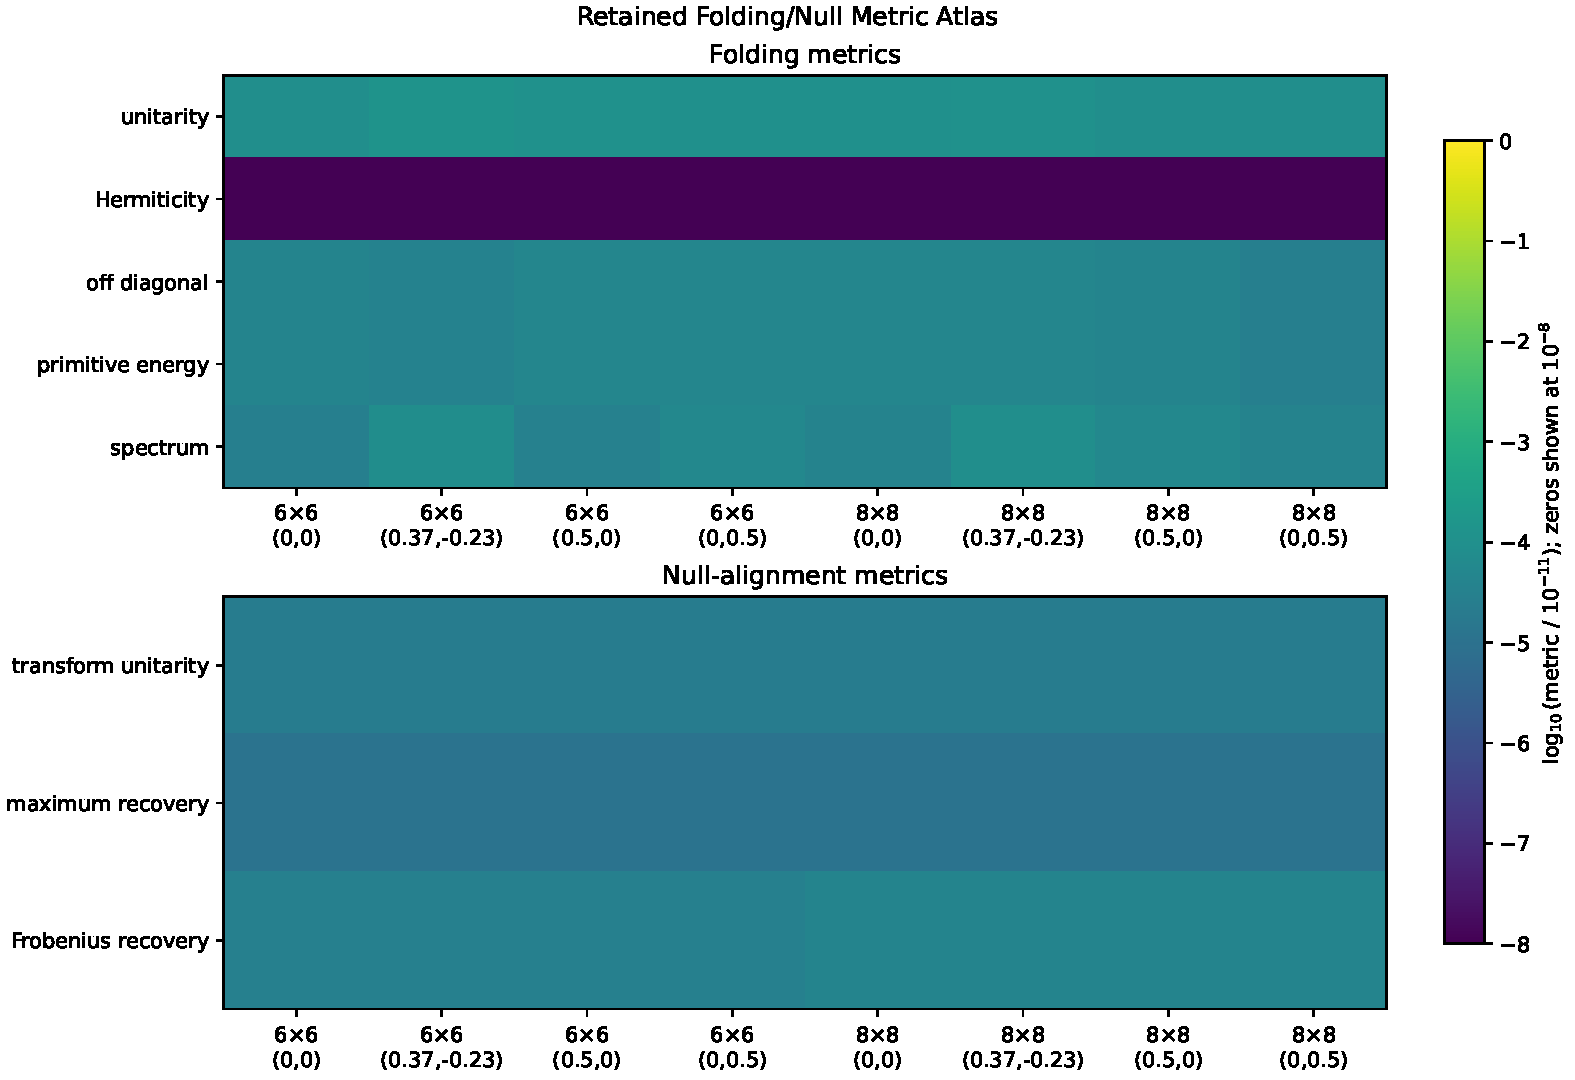
\includegraphics[width=0.96\textwidth]{../figures-v3/folding-null-metric-atlas.pdf}
  \caption{V02: every retained folding and null-alignment metric shown separately,
  normalized by the prospective $10^{-11}$ criterion.  The existing maximum-residual
  summary is not used to conceal individual channels.}
  \label{fig:folding-null-metric-atlas}
\end{figure}

\begin{figure}[p]
  \centering
  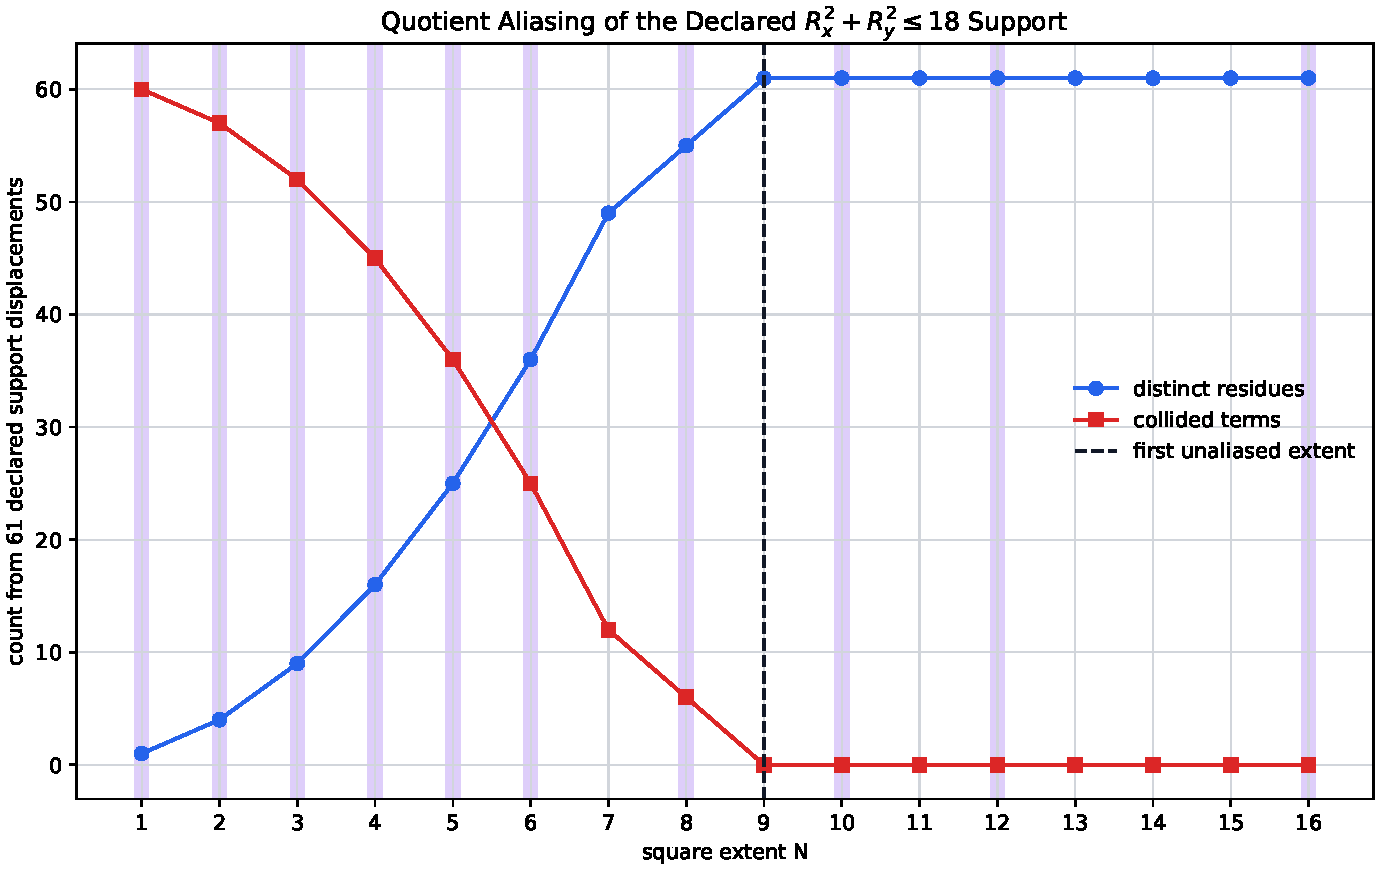
\includegraphics[width=0.96\textwidth]{../figures-v3/parent-support-collisions.pdf}
  \caption{P02: distinct quotient residues and collided declared radius-18 parent
  support terms versus square extent.  Purple marks identify retained square controls;
  this is support geometry rather than an operator result.}
  \label{fig:parent-support-collisions}
\end{figure}

\begin{figure}[p]
  \centering
  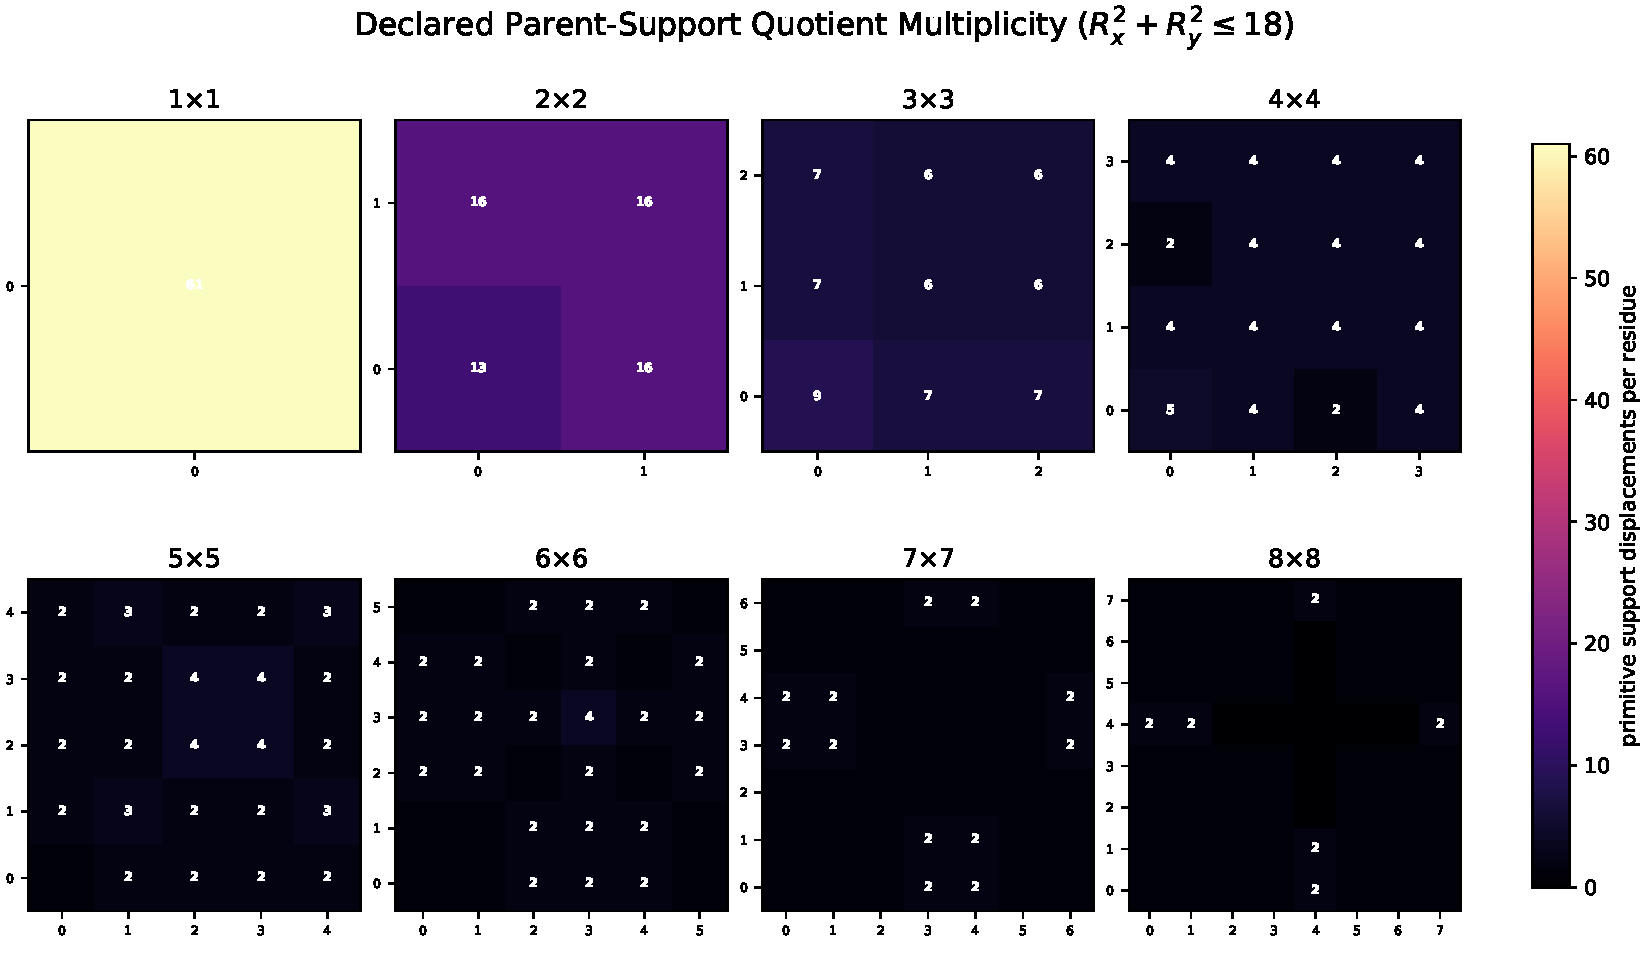
\includegraphics[width=0.98\textwidth]{../figures-v3/parent-support-equivalence-maps.pdf}
  \caption{P03: residue multiplicities for the 61 declared radius-18 parent-support
  displacements on the $1\times1$ through $8\times8$ quotients.  Numbers mark collided
  multiplicities greater than one.}
  \label{fig:parent-support-equivalence}
\end{figure}

\begin{figure}[p]
  \centering
  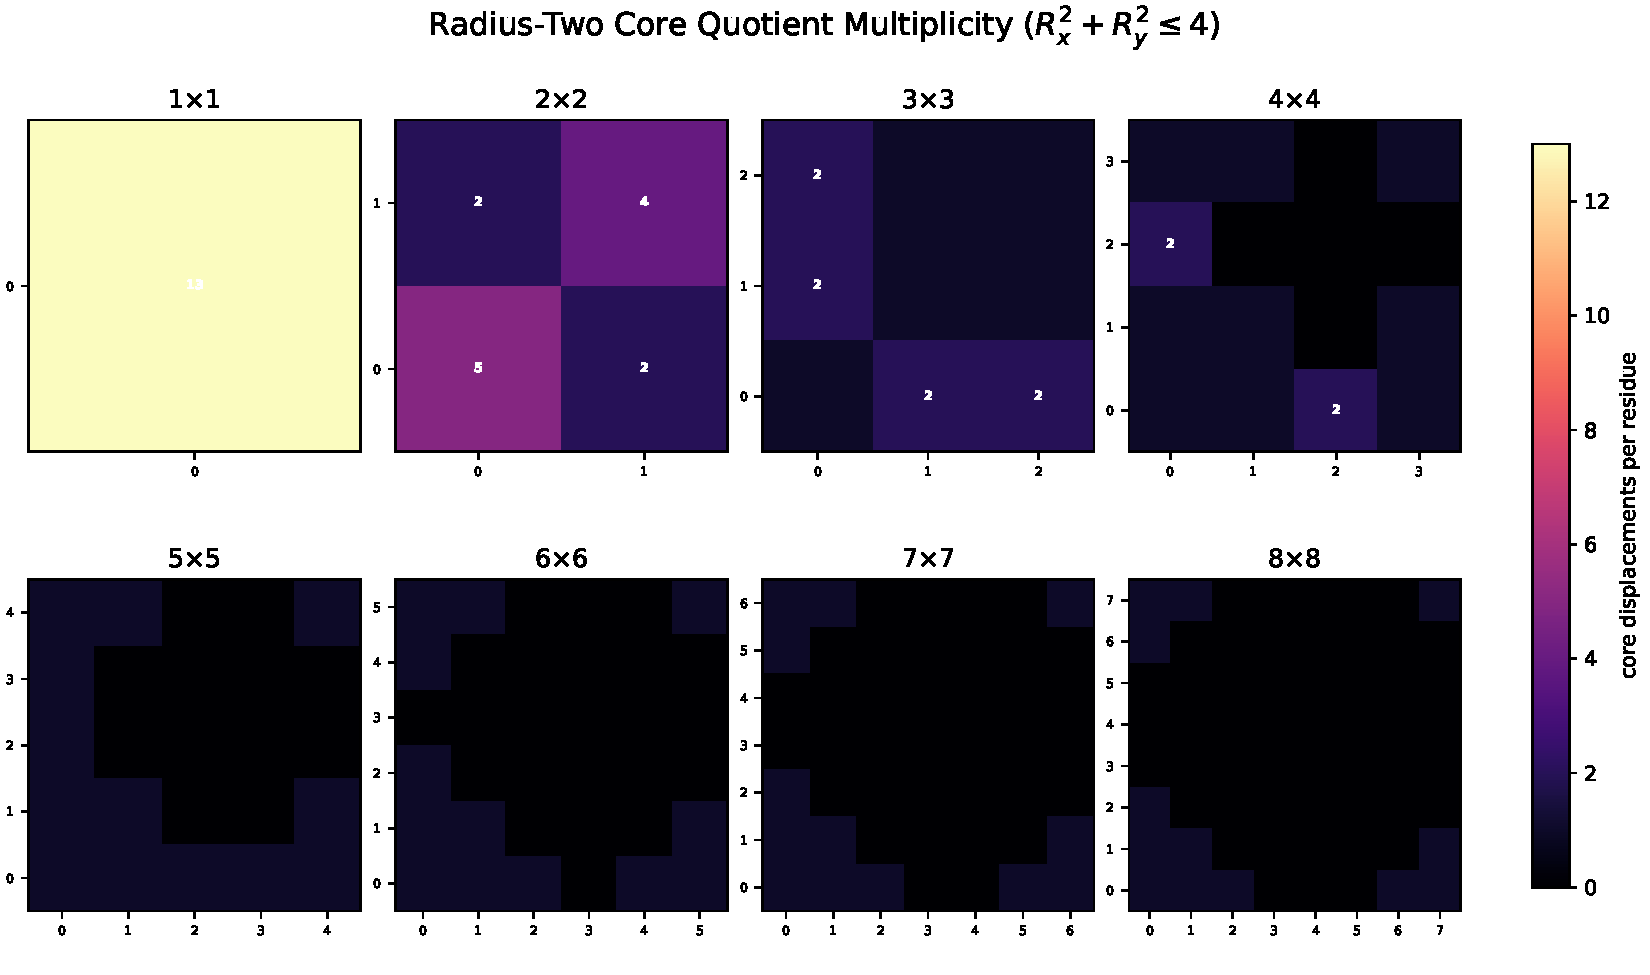
\includegraphics[width=0.98\textwidth]{../figures-v3/radius-two-core-equivalence-maps.pdf}
  \caption{P04: quotient multiplicities for the 13 integer displacements in the
  radius-two analysis core.  The plot describes aliasing of declared support geometry,
  not a calculated perturbation.}
  \label{fig:radius-two-core-equivalence}
\end{figure}

\begin{figure}[p]
  \centering
  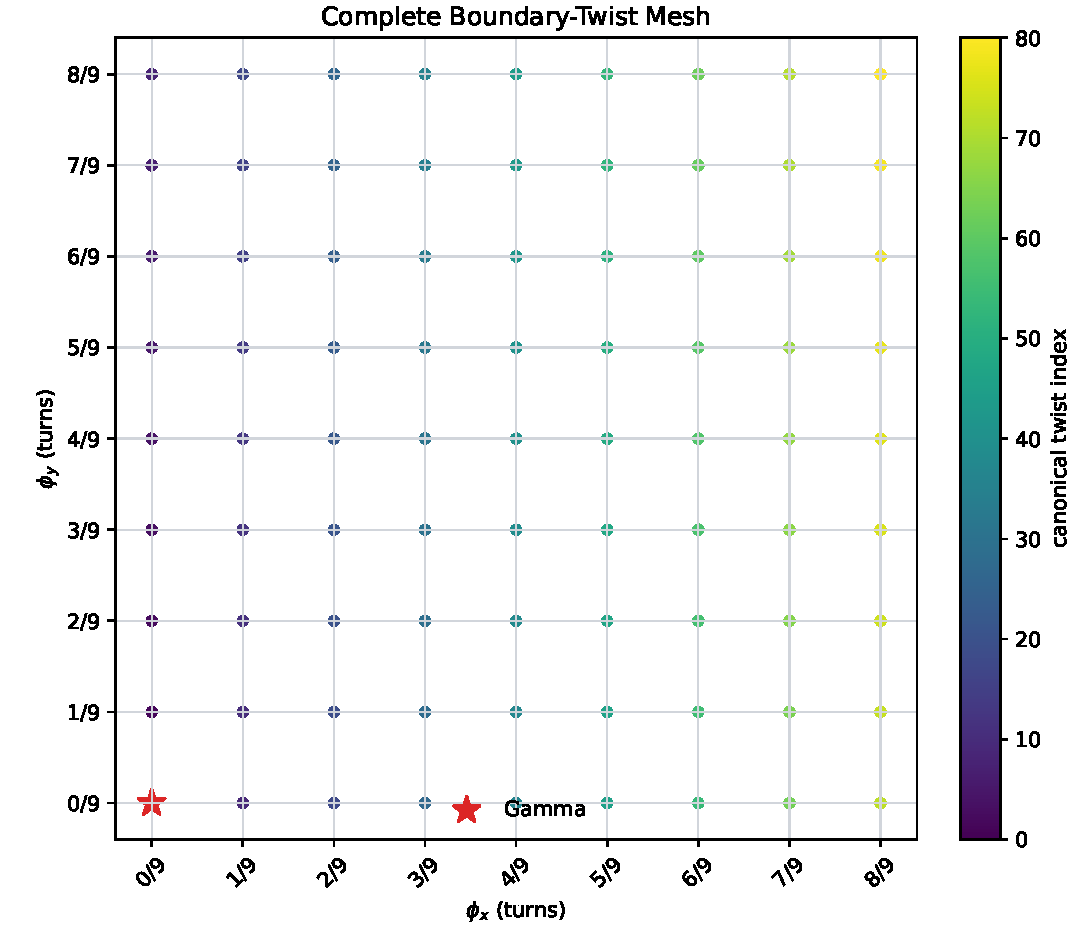
\includegraphics[width=0.82\textwidth]{../figures-v3/boundary-twist-mesh.pdf}
  \caption{P05: the complete $9\times9$ unweighted boundary-twist mesh in canonical
  first-axis-outer, second-axis-inner order.  It is not weighted reciprocal-space
  sampling.}
  \label{fig:boundary-twist-mesh}
\end{figure}

\begin{figure}[p]
  \centering
  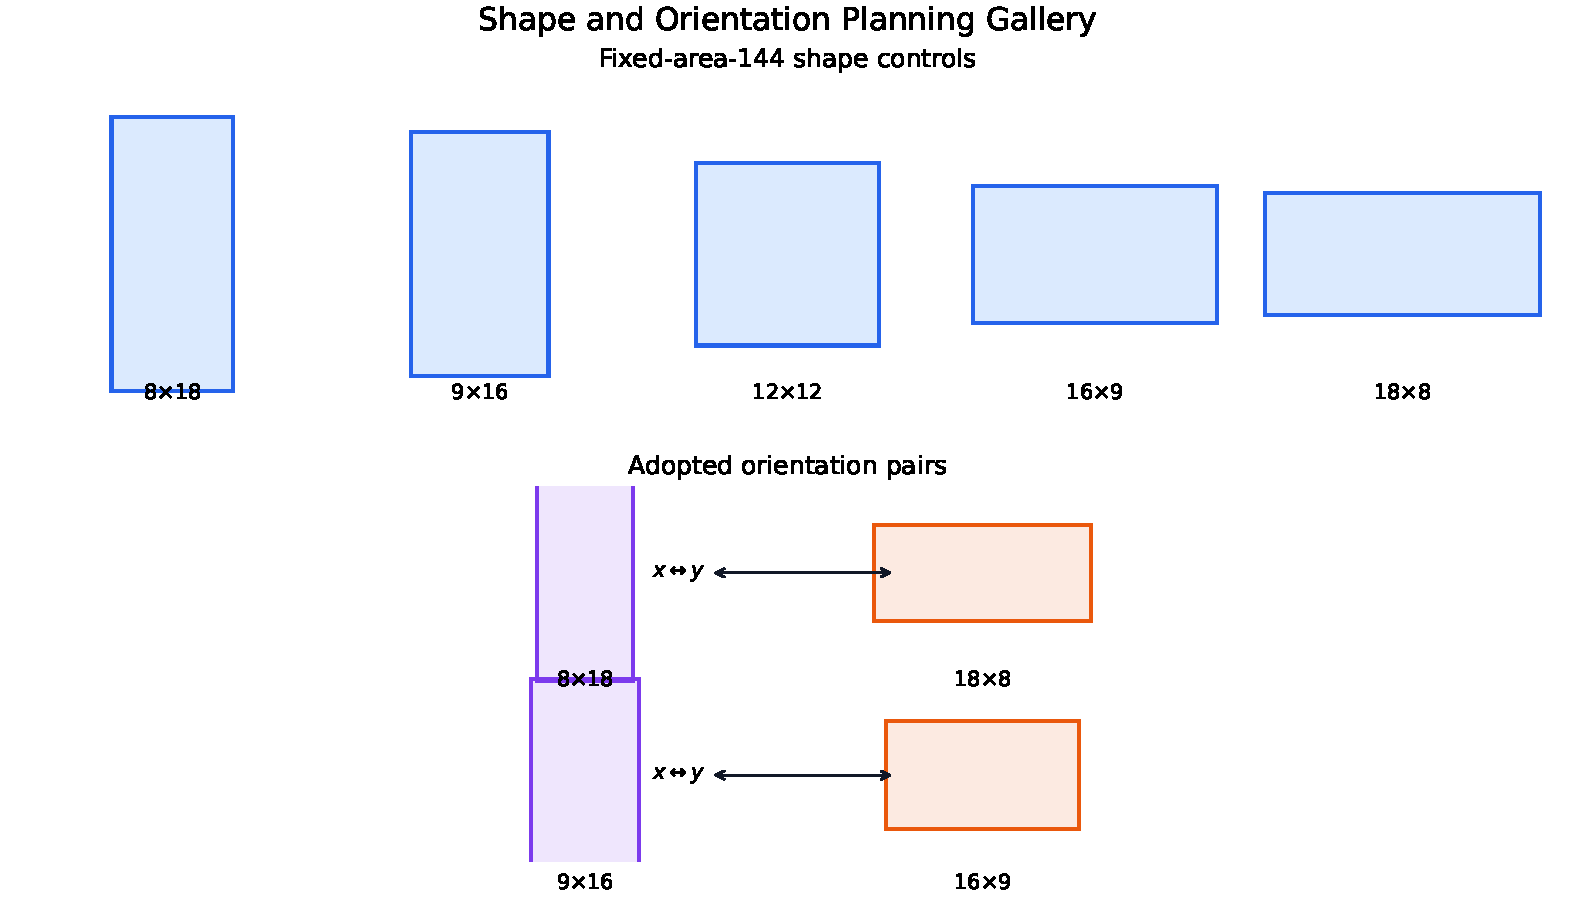
\includegraphics[width=0.94\textwidth]{../figures-v3/shape-orientation-gallery.pdf}
  \caption{P06: the five fixed-area-144 rectangles and the two frozen axis-swap
  orientation pairs.  Equal area does not imply represented compatibility or a zero
  same-parent contrast.}
  \label{fig:shape-orientation-gallery}
\end{figure}

\begin{figure}[p]
  \centering
  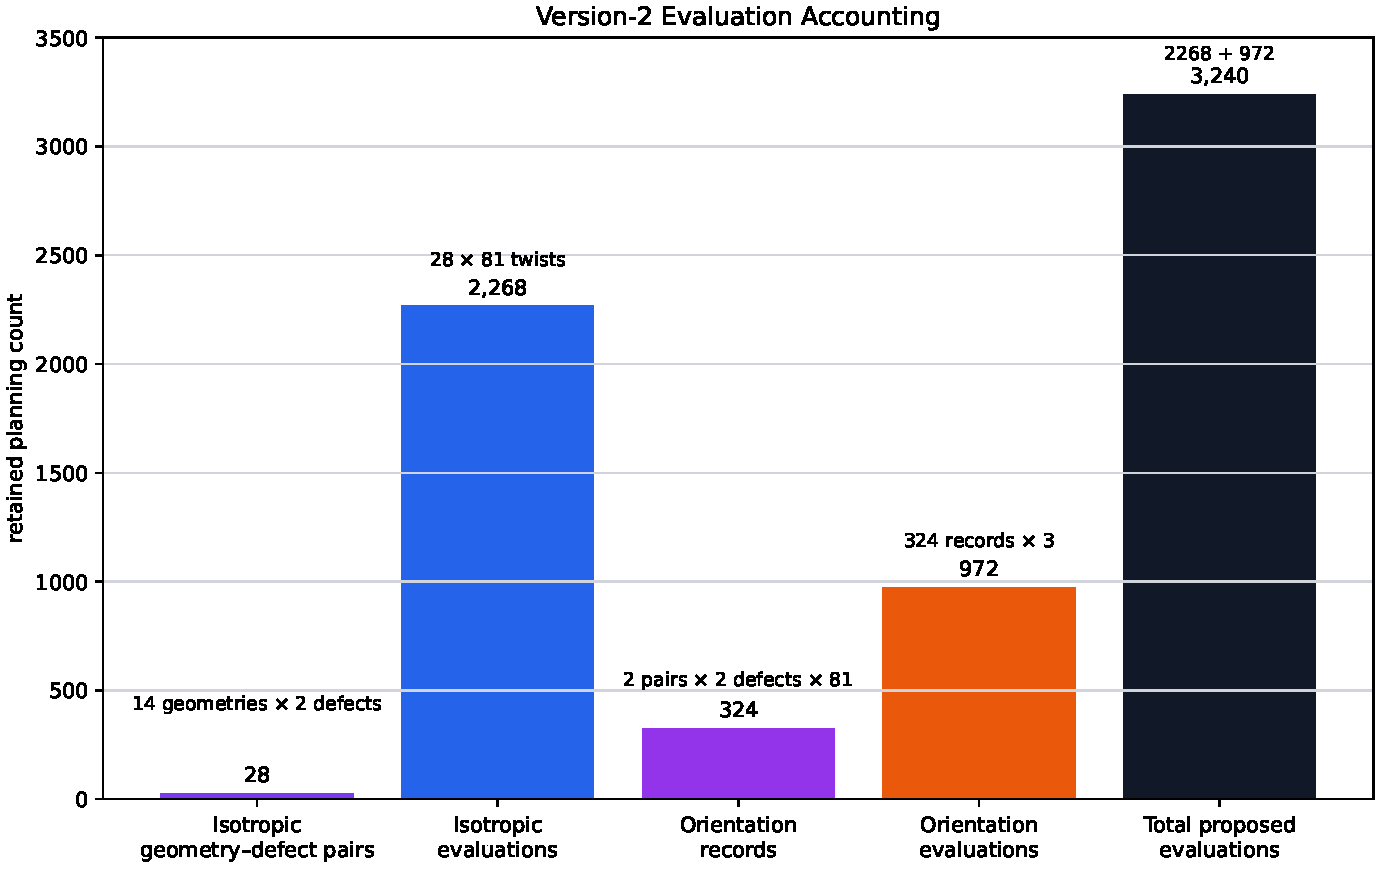
\includegraphics[width=0.92\textwidth]{../figures-v3/evaluation-accounting.pdf}
  \caption{P07: exact version-two planning arithmetic.  The 3,240 evaluations remain
  proposed and unexecuted.}
  \label{fig:evaluation-accounting}
\end{figure}

\begin{figure}[p]
  \centering
  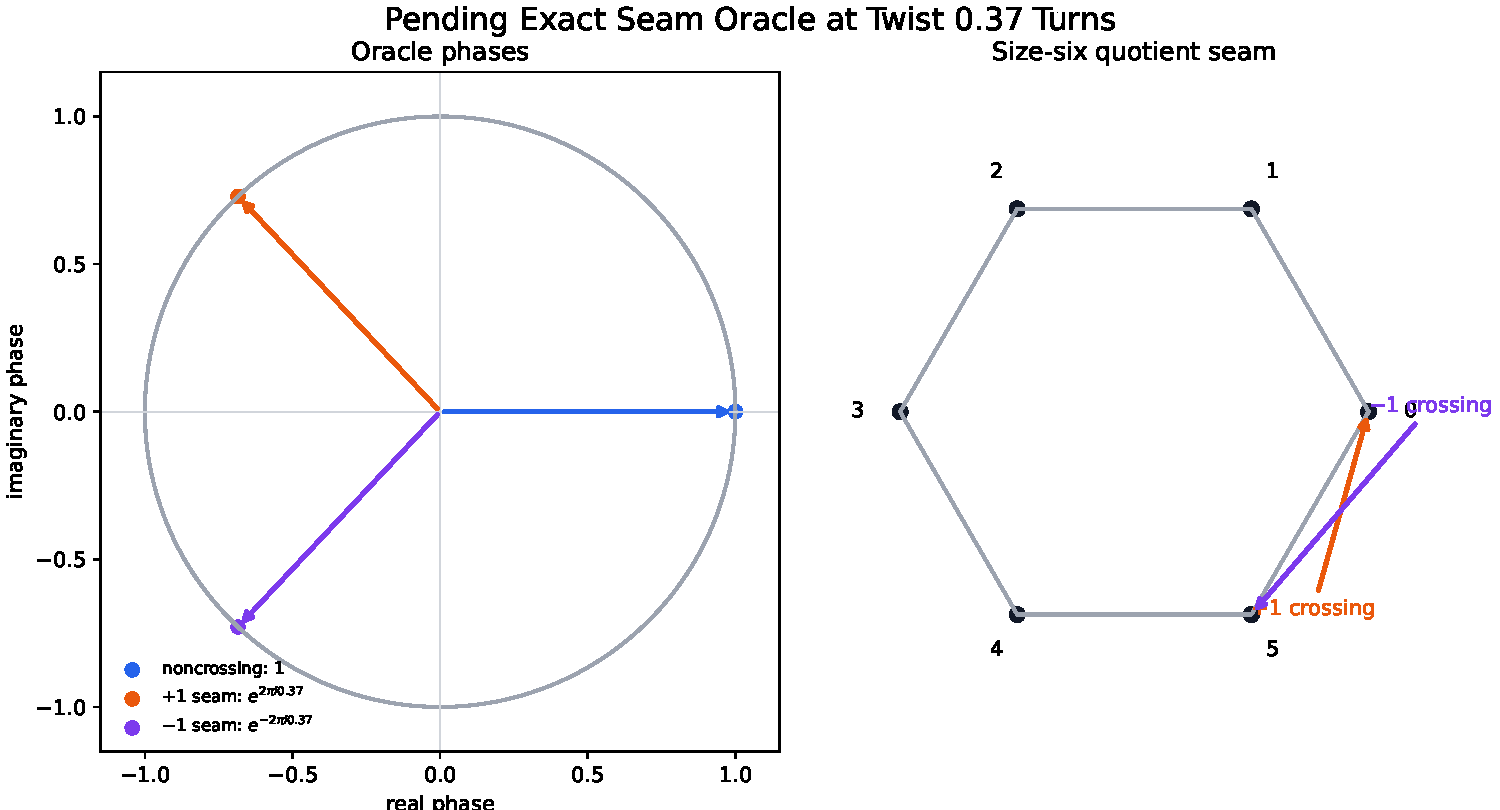
\includegraphics[width=0.94\textwidth]{../figures-v3/seam-oracle-phases.pdf}
  \caption{V03 planning diagram: the exact expected noncrossing, positive-seam, and
  negative-seam phases at $0.37$ turns for a size-six quotient.  This diagram defines
  the pending oracle; it does not claim that a new oracle execution occurred.}
  \label{fig:seam-oracle-phases}
\end{figure}

\begin{figure}[p]
  \centering
  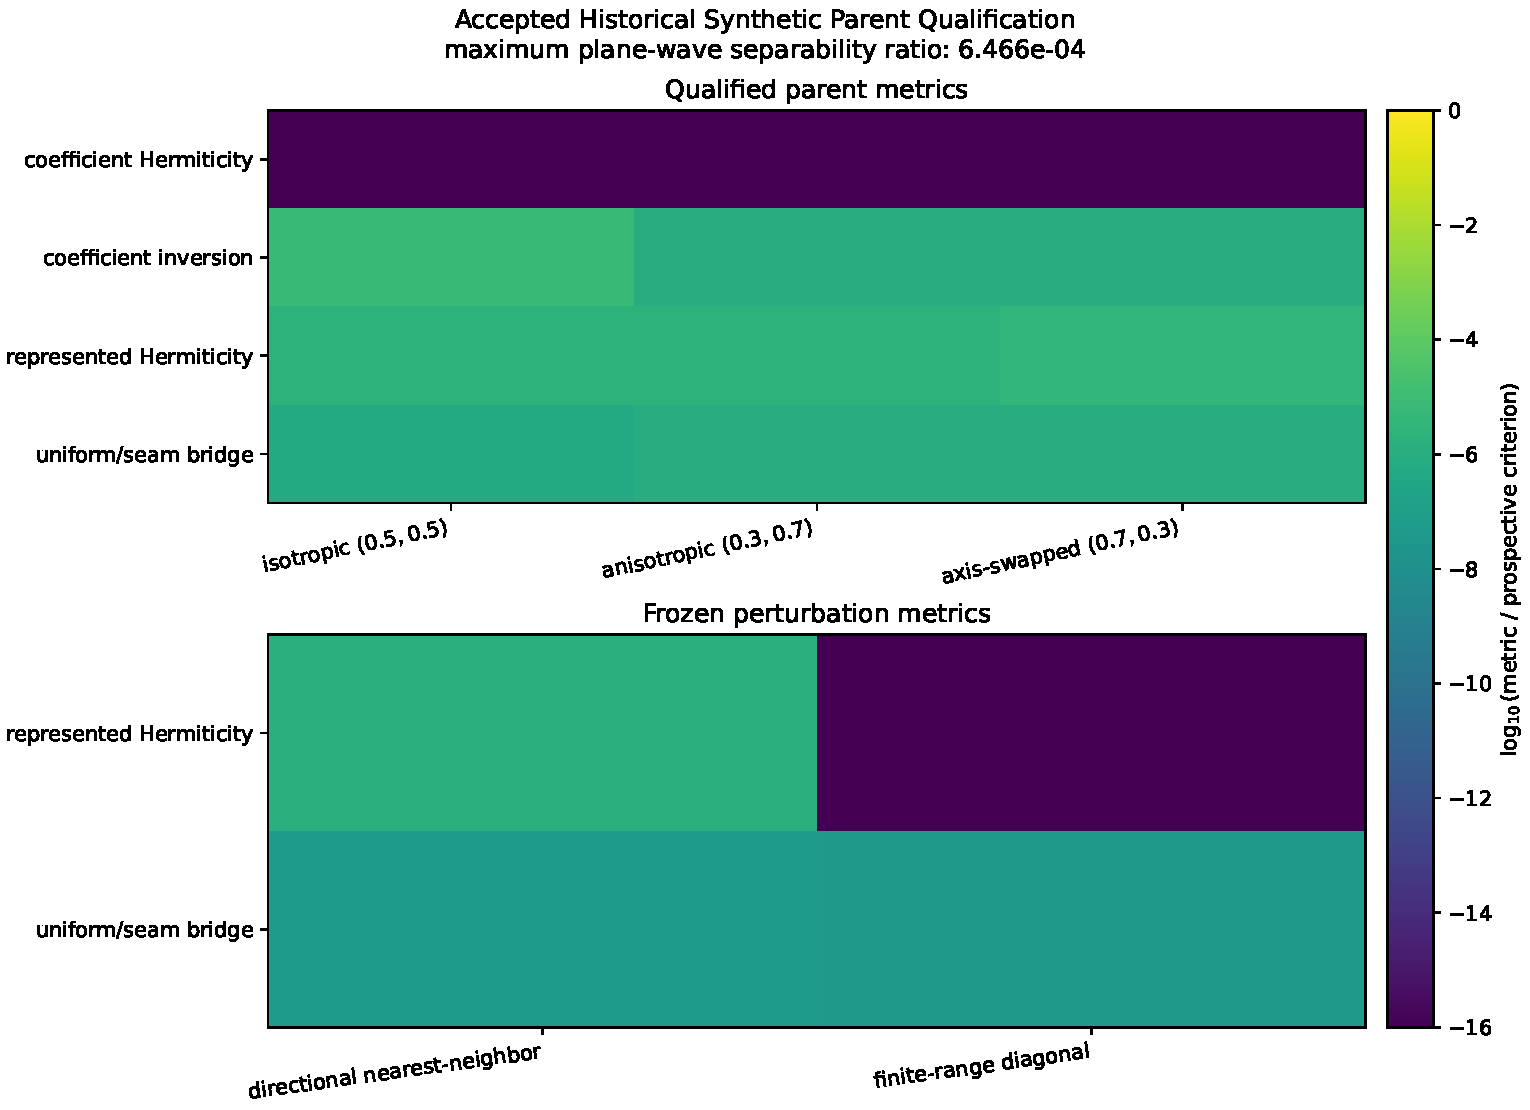
\includegraphics[width=0.96\textwidth]{../figures-v3/parent-qualification-metric-atlas.pdf}
  \caption{Retained parent-qualification metric atlas.  Parent and frozen-perturbation
  channels are normalized separately by their prospective criteria; the plane-wave
  separability maximum is reported as an additional ratio rather than pooled into the
  heatmap.}
  \label{fig:parent-qualification-metric-atlas}
\end{figure}

\begin{figure}[p]
  \centering
  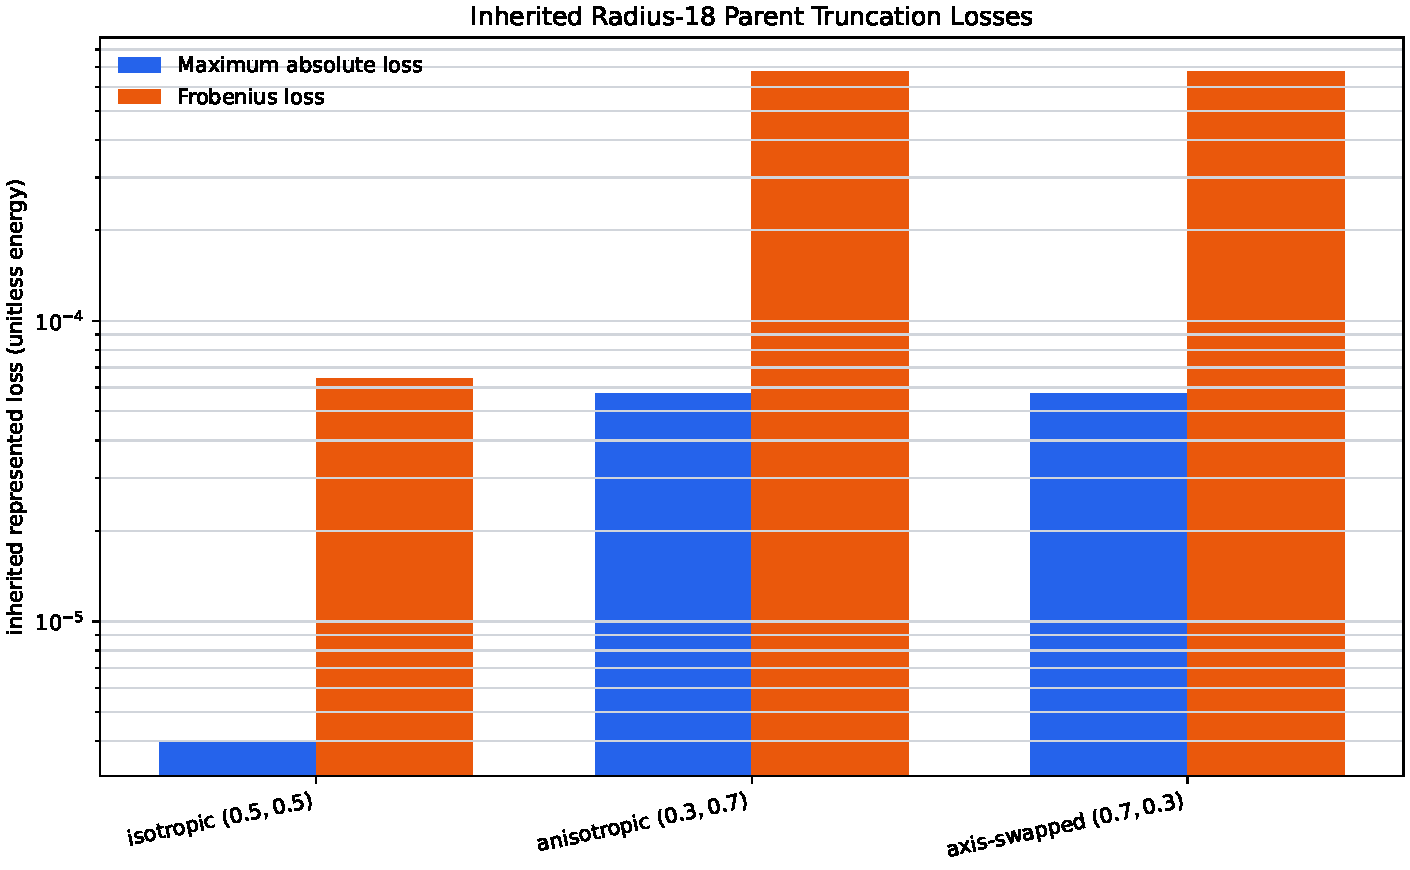
\includegraphics[width=0.90\textwidth]{../figures-v3/parent-truncation-losses.pdf}
  \caption{Inherited radius-18 maximum and Frobenius truncation losses for the three
  qualified synthetic parents.  These are source-to-compact parent losses, not
  production-versus-verification defects.}
  \label{fig:parent-truncation-losses}
\end{figure}

\begin{figure}[p]
  \centering
  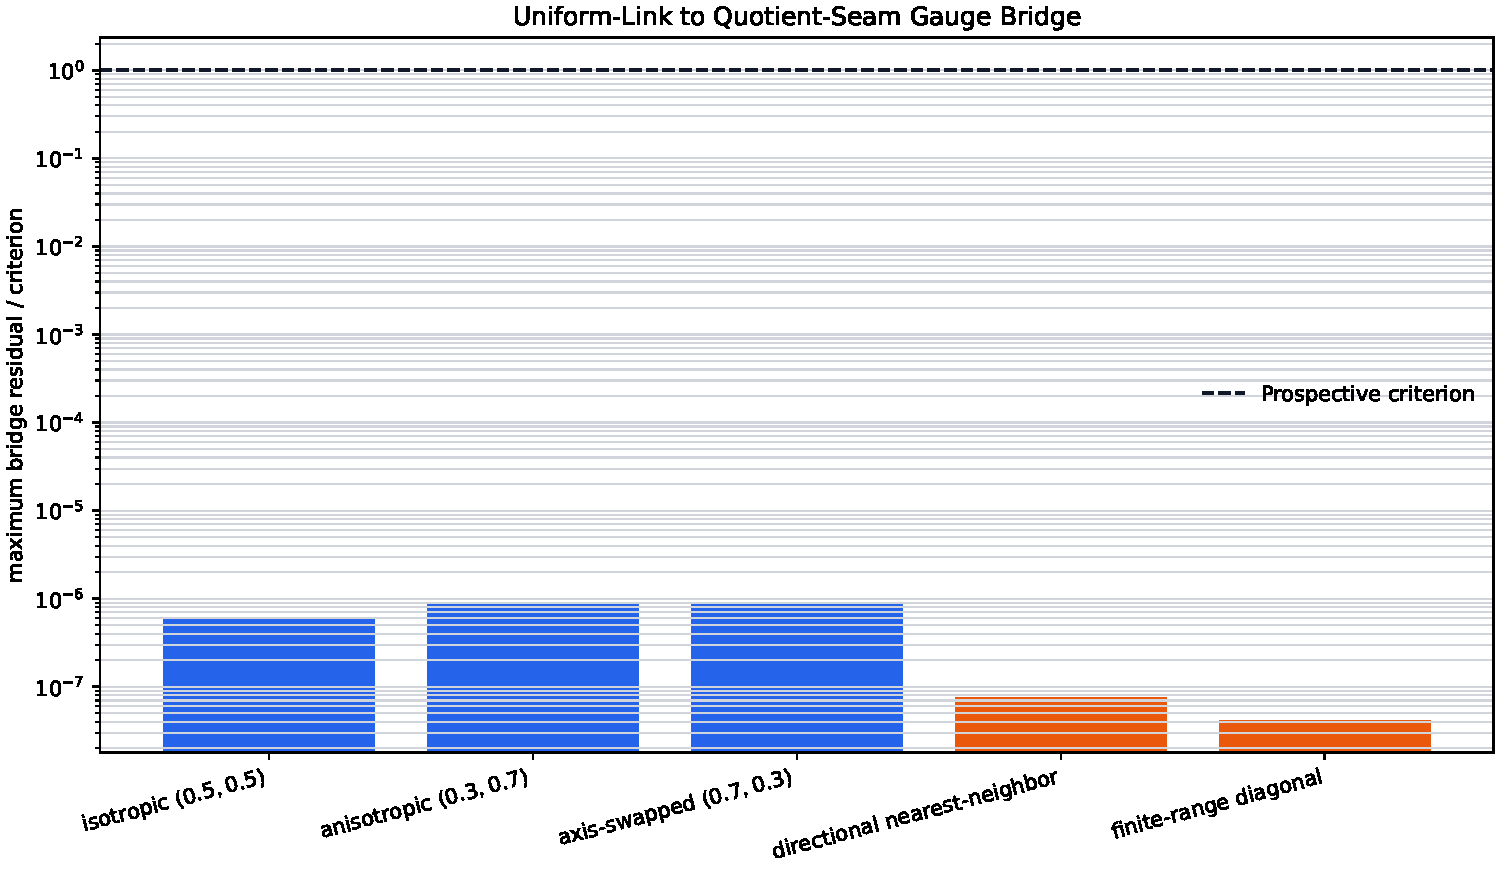
\includegraphics[width=0.94\textwidth]{../figures-v3/parent-gauge-bridge-residuals.pdf}
  \caption{V04: retained uniform-link to quotient-seam bridge residuals for all three
  qualified parents and both frozen perturbation inventories.}
  \label{fig:parent-gauge-bridge-residuals}
\end{figure}

\begin{figure}[p]
  \centering
  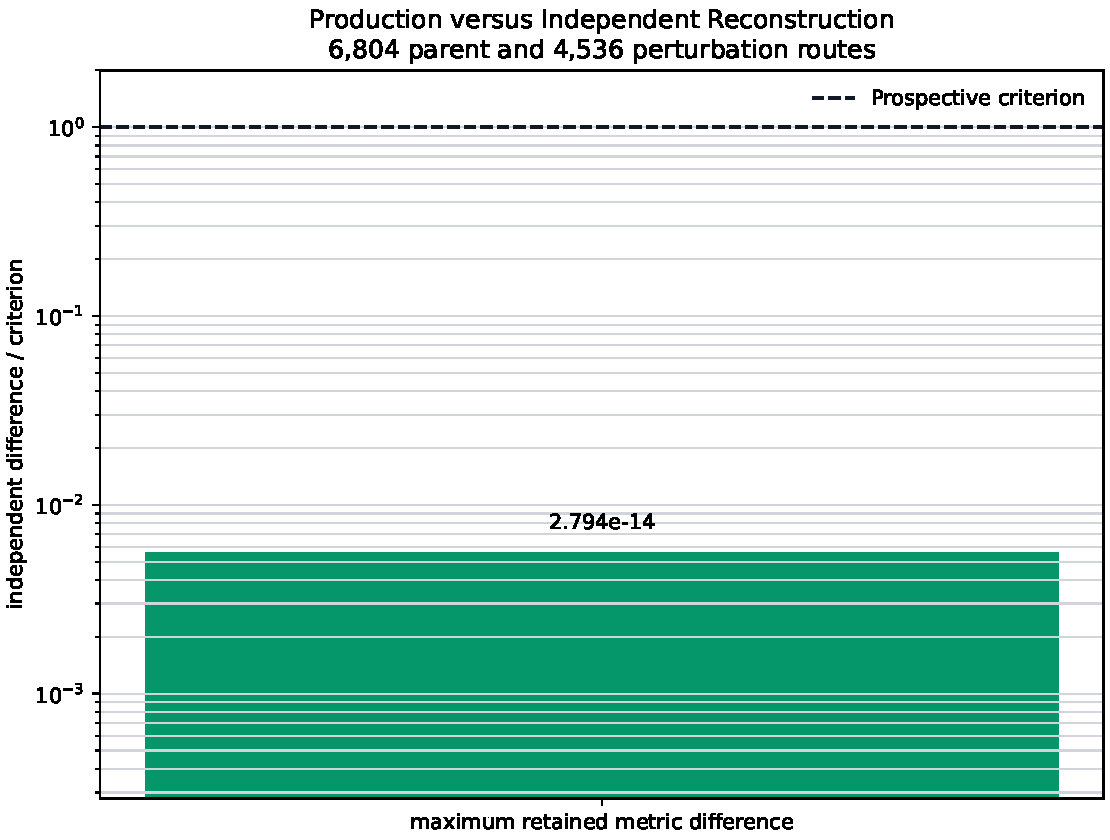
\includegraphics[width=0.82\textwidth]{../figures-v3/parent-independent-reconstruction.pdf}
  \caption{V05: aggregate maximum metric difference between production and independent
  reconstruction over 6,804 parent and 4,536 perturbation routes.  The retained record
  does not expose a per-case residual distribution.}
  \label{fig:parent-independent-reconstruction}
\end{figure}

\begin{figure}[p]
  \centering
  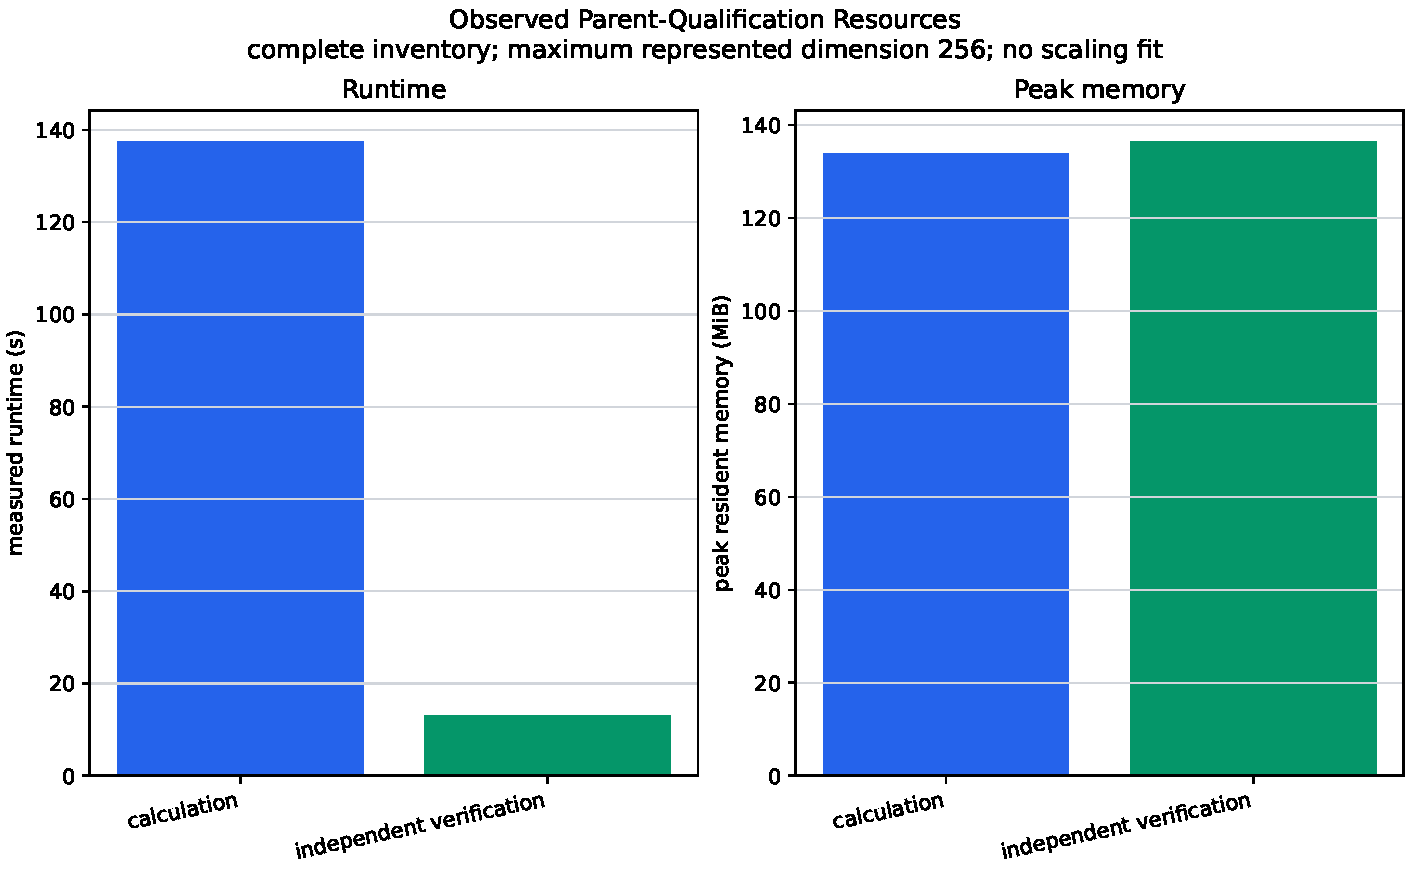
\includegraphics[width=0.94\textwidth]{../figures-v3/parent-resource-observation.pdf}
  \caption{V06: measured runtime and peak resident memory for calculation and
  independent verification of the complete qualification inventory.  These two
  aggregate observations do not define a dimension-scaling law.}
  \label{fig:parent-resource-observation}
\end{figure}
\clearpage

\section{Diagnostics and degeneracy policy}

Compatible cases may report maximum-entry, Frobenius, spectral, radius-two core,
exterior, core--exterior, and spatial-shell operator diagnostics.  Spectral and state
diagnostics may include host-edge-referenced binding energy, below-edge state count,
defect-band center and width, eigenpair residual, projector fidelity, core probability,
inverse participation ratio, separate $x/y$ RMS radii, and quadrupole anisotropy.  A
no-bound-state case is retained; unavailable state-only metrics are not replaced with
zeros.

Individual vectors inside a degenerate cluster are not accepted observables.  Cluster
ranks are selected from the parent spectrum using adjacent-gap threshold $10^{-8}$ in
the declared energy unit.  For orthonormal bases $V$ and $W$, the primary objects are
projectors $VV^\dagger$ and $WW^\dagger$, principal angles, and the minimum singular
value of $V^\dagger W$.  Individual-vector requests stop with
\path{DEFECT_2D.DEGENERATE_PROJECTOR_REQUIRED}; alignment stops below minimum singular
value $0.5$.

\section{Error-channel separation}

The following remain separate: parent-model or parent-truncation error; represented-space
or discretization error; folding and boundary-gauge conversion error; site,
point-group, orbital, and energy-reference alignment error; finite-area effect;
fixed-area shape effect; orientation effect; boundary-phase effect; defect
model-reduction error; eigensolver residual; serialization or provenance error; and
total finite-model consequence.  No pooled scalar error may conceal these channels.
Restoring full support converges to the fixed represented parent, not to an unrepresented
physical or DFT parent.  The retained error report is therefore a channel vector
\begin{equation}
  \begin{aligned}
  \mathbf e=(&e_{\mathrm{parent}},e_{\mathrm{representation}},
   e_{\mathrm{gauge}},e_{\mathrm{alignment}},\\
   &e_{\mathrm{area}},e_{\mathrm{shape}},e_{\mathrm{orientation}},
   e_{\mathrm{twist}},\\
   &e_{\mathrm{reduction}},e_{\mathrm{eigensolver}},
   e_{\mathrm{provenance}}).
  \end{aligned}
\end{equation}
not a scalar sum.  An equation such as $e_{\mathrm{total}}=\sum_a e_a$ is forbidden
unless a separately reviewed model defines the dependence and normalization of every
term.

\section{Frozen criteria}

\begin{center}
\small
\begin{tabularx}{\textwidth}{Y>{\raggedleft\arraybackslash}p{0.28\textwidth}}
\toprule
\textbf{Quantity} & \textbf{Criterion} \\
\midrule
Folding and null-alignment algebraic absolute & $10^{-11}$ \\
Folding unitarity & $10^{-11}$ \\
Projector Frobenius & $10^{-10}$ \\
Symmetry or covariance absolute & $10^{-10}$ in declared energy unit \\
Minimum alignment singular value & $0.5$ \\
Degenerate adjacent gap & $10^{-8}$ in declared energy unit \\
Bound-state classification threshold & $10^{-10}$ in declared energy unit \\
Eigenpair residual & $10^{-10}$ in declared energy unit \\
Independent reconstruction relative & $10^{-10}$ \\
Final area-channel operator relative change & $10^{-3}$ \\
Final area-channel energy change divided by parent bandwidth & $10^{-3}$ \\
Final area-channel center or radius absolute change & $10^{-3}$ cells \\
\bottomrule
\end{tabularx}
\end{center}

Finite-domain criteria are reporting rules, not guarantees of convergence or scientific
acceptance.  A zero normalization denominator stops with
\path{DEFECT_2D.NONFINITE_DIAGNOSTIC}.  Workstream-specific stricter controls do not
silently replace criteria for other workstreams.

\section{Structured stops}

No extracted residual is returned after:
\begin{itemize}[leftmargin=*]
  \item \path{DEFECT_2D.PARENT_IDENTITY_MISMATCH};
  \item \path{DEFECT_2D.FOLDING_NOT_UNITARY};
  \item \path{DEFECT_2D.GEOMETRY_MISMATCH};
  \item \path{DEFECT_2D.BOUNDARY_PHASE_MISMATCH};
  \item \path{DEFECT_2D.SITE_MAP_UNRESOLVED};
  \item \path{DEFECT_2D.PHASE_GRAPH_DISCONNECTED};
  \item \path{DEFECT_2D.SUBSPACE_OVERLAP_TOO_SMALL};
  \item \path{DEFECT_2D.DEGENERATE_PROJECTOR_REQUIRED};
  \item \path{DEFECT_2D.ENERGY_REFERENCE_UNKNOWN}; or
  \item \path{DEFECT_2D.NONFINITE_DIAGNOSTIC}.
\end{itemize}
Process failure, represented incompatibility, numerical criterion failure,
nonconvergence, and no-bound-state outcomes are distinct statuses.

\section{Production and independent verification}

Production and verification remain separate implementations.  The current producer uses
the maintained quotient-seam constructor and explicit finite folding.  The verifier
reconstructs one-dimensional seam matrices, Kronecker products, Fourier factors,
primitive energies, and the known inverse through separate arithmetic and does not
import the producer script.

A future finite-domain producer may use a centered uniform-link gauge only when declared.
Its verifier must use quotient-seam construction and apply the explicit site-diagonal
gauge bridge before comparison.  Gauge-equivalent routes are not independent estimates
and are not averaged or allowed to vote.

Every verifier authenticates serialized inputs and retained results before semantic
comparison and rejects missing cases, changed thresholds, changed ordering, discarded
failures, noncanonical bytes where canonical encoding is required, and source or
artifact digest mismatches.

\begin{figure}[htbp]
  \centering
  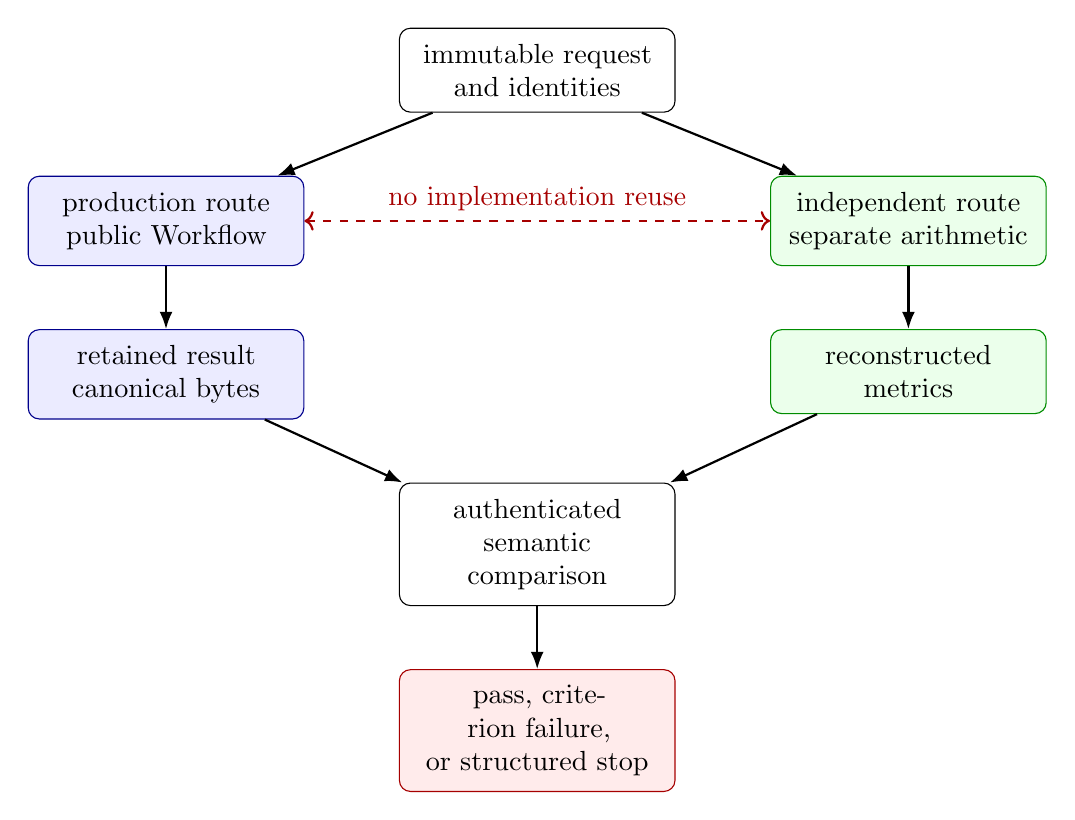
\begin{tikzpicture}[node distance=8mm and 12mm]
    \node[protocolbox] (request) {immutable request\\and identities};
    \node[evidencebox,below left=of request] (prod)
      {production route\\public Workflow};
    \node[verifybox,below right=of request] (verify)
      {independent route\\separate arithmetic};
    \node[evidencebox,below=of prod] (result)
      {retained result\\canonical bytes};
    \node[verifybox,below=of verify] (recon)
      {reconstructed\\metrics};
    \node[protocolbox,below right=of result] (compare)
      {authenticated semantic\\comparison};
    \node[stopbox,below=of compare] (status)
      {pass, criterion failure,\\or structured stop};
    \draw[protocolarrow] (request) -- (prod);
    \draw[protocolarrow] (request) -- (verify);
    \draw[protocolarrow] (prod) -- (result);
    \draw[protocolarrow] (verify) -- (recon);
    \draw[protocolarrow] (result) -- (compare);
    \draw[protocolarrow] (recon) -- (compare);
    \draw[protocolarrow] (compare) -- (status);
    \draw[red!65!black,dashed,thick,<->] (prod) -- node[above,sloped]
      {no implementation reuse} (verify);
  \end{tikzpicture}
  \caption{Production and independent-verification boundary.  Shared immutable inputs
  are allowed; production construction and arithmetic are not imported by verification.}
  \label{fig:verification-boundary}
\end{figure}

\section{Workflow and retention contract}

Each maintained workstream has separate calculation and independent-verification
Workflows.  A calculation script does not bypass its public Workflow, and a verification
script does not invoke the calculation route.

A retained package includes, as applicable, a separately serialized immutable request,
source and artifact SHA-256 identities, repository revision and dirty-state disposition,
software versions, execution status and resource observations, compact results including
failed and unavailable outcomes, independent verification, checksum manifest, and a
report of claims and nonclaims.  Dense matrices are reconstructed rather than retained
unless a separately reviewed small-matrix artifact is necessary.  Scripts and packages
use no-overwrite behavior.  Superseded evidence is not silently rewritten to match new
code.

\section{Parent-capability parity gate}

The symbolic planning identifiers
\path{isotropic_lambda_0p5_0p5_0},
\path{anisotropic_lambda_0p3_0p7_0}, and
\path{anisotropic_lambda_0p7_0p3_0} are instantiated only by the separately retained
\path{executions/parent-qualification-v1/} package.  That package binds accepted
historical synthetic source identities, the scalar rank-one state space and
$x$-outer/$y$-inner ordering, uniform-link and quotient-seam gauges, the complete
$9\times9$ twist mesh, unitless energy and the accepted parent zero, radius-18 support,
inherited truncation losses, both frozen Hermitian perturbations, public production
constructors, direct independent seam/gauge reconstruction, prospective criteria,
resource bounds, and no-overwrite retention.

The qualification evaluates fourteen unique shapes, 6,804 parent route constructions,
and 4,536 perturbation route constructions.  Its calculation criteria and independent
reconstruction pass; the maximum aggregate verification difference is
$2.79359868571305\times10^{-14}$.  An additive read-only audit authenticates the
compact and full isotropic projections, anisotropic parameters, historical compact
parent identities, all four source-object hashes, implementation modules, scripts, and
installed package versions without replacing the original manifest.  This closes the
calculation-local parent-definition
and represented-construction portion of the gate for these exact synthetic parents.
It does not establish material validation, finite-domain convergence, isolated-defect
behavior, uncertainty quantification, or authority to execute the 3,240 proposed defect
evaluations.  The broader periodic2d capability-parity program, successor campaign
contracts, and prospective absolute isolation thresholds remain separate open gates.

\section{Authorization and resource policy}

Under the current human instruction, documentation, execution-free contract extraction,
authored fixtures, software tests, reconstruction of retained compact evidence, and the
bounded local parent qualification are in scope.  The parent-qualification instruction
has been consumed by the retained version-one package; it did not authorize the defect
campaign.  This document itself does not authorize protected or external calculation.
Before an authorized operator-producing run, the operator receives the entry point,
exact input system, matrix dimensions and case count, output package, estimated runtime
and memory, and external-storage or network disposition.

Historical planning estimates are: maximum dimension 64, 120 seconds, and 2 GiB for
Folding and Null-Alignment Controls; maximum dimension 64 for authored Defect-Model
Discrimination controls; and maximum scalar dimension 288, approximately 2 GiB, and an
estimated 20-minute serial runtime for the superseded version-1 Finite-Domain
Sensitivity inventory.  The retained parent qualification measured
$137.36745366686955$ seconds and $140410880$ peak resident bytes for calculation, and
$13.155915041919798$ seconds and $142983168$ peak resident bytes for independent
verification, within its 600-second and 2-GiB post-computation bounds.  No runtime
estimate has been adopted for the expanded version-2 defect inventory.  These
observations are not hard containment guarantees or successor execution authority.

\section{Change control and acceptance}

Any change to parent identity, rank, geometry, gauge, twist mesh, support, defect
strength, attack, model order, threshold, normalization, comparison channel, or case
inventory requires a versioned revision before calculation.

Acceptance is layered:
\begin{enumerate}[leftmargin=*]
  \item software verification establishes contract, serialization, Workflow, and failure
    behavior;
  \item numerical verification establishes agreement with independent reconstruction
    for the represented synthetic problem;
  \item scientific validation requires an independently qualified physical parent and
    is absent;
  \item uncertainty quantification is absent unless separately designed and executed;
    and
  \item publication qualification requires independent reconstruction and explicit
    human review beyond a passing package.
\end{enumerate}
A workstream pass does not authorize the next workstream, publication, release,
submission, commit, push, merge, or protected computation.

\section{Direct technique references}

\begin{itemize}[leftmargin=*]
  \item F. Bloch, ``\"Uber die Quantenmechanik der Elektronen in
    Kristallgittern,'' \emph{Zeitschrift f\"ur Physik} \textbf{52}, 555--600
    (1929), DOI \href{https://doi.org/10.1007/BF01339455}{10.1007/BF01339455}.
  \item P. H. Sch\"onemann, ``A Generalized Solution of the Orthogonal Procrustes
    Problem,'' \emph{Psychometrika} \textbf{31}, 1--10 (1966), DOI
    \href{https://doi.org/10.1007/BF02289451}{10.1007/BF02289451}.
  \item N. J. Higham, ``Computing the Polar Decomposition---with Applications,''
    \emph{SIAM Journal on Scientific and Statistical Computing} \textbf{7},
    1160--1174 (1986), DOI
    \href{https://doi.org/10.1137/0907079}{10.1137/0907079}.
  \item Q. Niu, D. J. Thouless, and Y.-S. Wu, ``Quantized Hall Conductance as a
    Topological Invariant,'' \emph{Physical Review B} \textbf{31}, 3372--3377
    (1985), DOI
    \href{https://doi.org/10.1103/PhysRevB.31.3372}{10.1103/PhysRevB.31.3372}.
\end{itemize}
These references support folding, finite-boundary, alignment, and subspace techniques;
they do not support retained numerical values or material claims.

\section{Current conclusions and non-results}

The retained evidence supports only that the authored rank-one parent folds correctly
for eight shape/twist cases within prospective criteria; the declared translation,
site-phase, and energy-reference attack recovers the null perturbation; independent
arithmetic reconstructs those metrics; and the three exact accepted historical
synthetic parents and two frozen perturbation inventories satisfy the declared
represented construction, Hermiticity, symmetry, gauge-bridge, source-identity, and
independent-reconstruction criteria over all fourteen planned shapes and 81 twists.
The exact Finite-Domain Sensitivity inventory can also be generated and authenticated
without executing its proposed defect evaluations.  It identifies $10\times10$ as the
first support-unaliased candidate for a future isolated-defect-like size assessment,
but selects no adequate size.

It does not establish completeness of the historical folding/null lifecycle; operator
results from Onsite Extraction and Covariance Controls, Defect-Model Discrimination,
Finite-Domain Sensitivity, or Composite-Subspace Extension; physical or material parent
adequacy; finite-size convergence; isolated-defect behavior; material transfer; a
validated physical defect Hamiltonian; scientific validation; or uncertainty bounds.

\end{document}
